\documentclass[11pt]{article}

\usepackage{cite}
\usepackage{amsmath,amssymb,amsfonts}
\usepackage{algorithmic}
\usepackage{graphicx}
\usepackage{textcomp}
\usepackage{xcolor}
\usepackage{booktabs}
\usepackage{caption}
\usepackage{xspace}
\usepackage{pdfpages}
\usepackage[T1]{fontenc}
\usepackage{float}
\usepackage{titlesec}
\usepackage{natbib}
\usepackage{hyperref}
\usepackage{multicol}
\usepackage{mwe}
\usepackage[utf8]{inputenc}
\usepackage{geometry}
\usepackage[table,xcdraw]{xcolor}
\usepackage[a4paper, total={5.2in, 8in}]{geometry} % adjust margins 
\usepackage{enumitem}


% removes first empty page  
\usepackage{atbegshi}
\AtBeginDocument{\AtBeginShipoutNext{\AtBeginShipoutDiscard}}


\begin{document}

% tex files 
\pagenumbering{gobble}

\newgeometry{left=2cm, right=0.2cm, top=1cm, bottom=-8cm}

\hspace{3.3cm}
\includegraphics[width = 0.5\linewidth]{images/itulogo.jpg}    

\vspace{1.5cm}

\noindent \textcolor{gray}{\huge{Exam Submission}}

\noindent \Huge{DevOps, Software Evolution\\ and Software Maintenance} \newline

%\vspace{0.2cm}

\normalsize
\noindent \textbf{Group S} \newline
Emiliano Gustavo Giusto (emgi@itu.dk), \newline
Ingrid Maria Christensen (inch@itu.dk),\newline
Matêj Basta (bact@itu.dk), \newline
Melissa Høegh Marcher (mhom@itu.dk), \newline
Nicholas Gioachini (ngio@itu.dk) \newline \newline
Course code: KSDSESM1KU \newline
May 2023

\begin{figure}[H]
  \makebox[\textwidth][r]{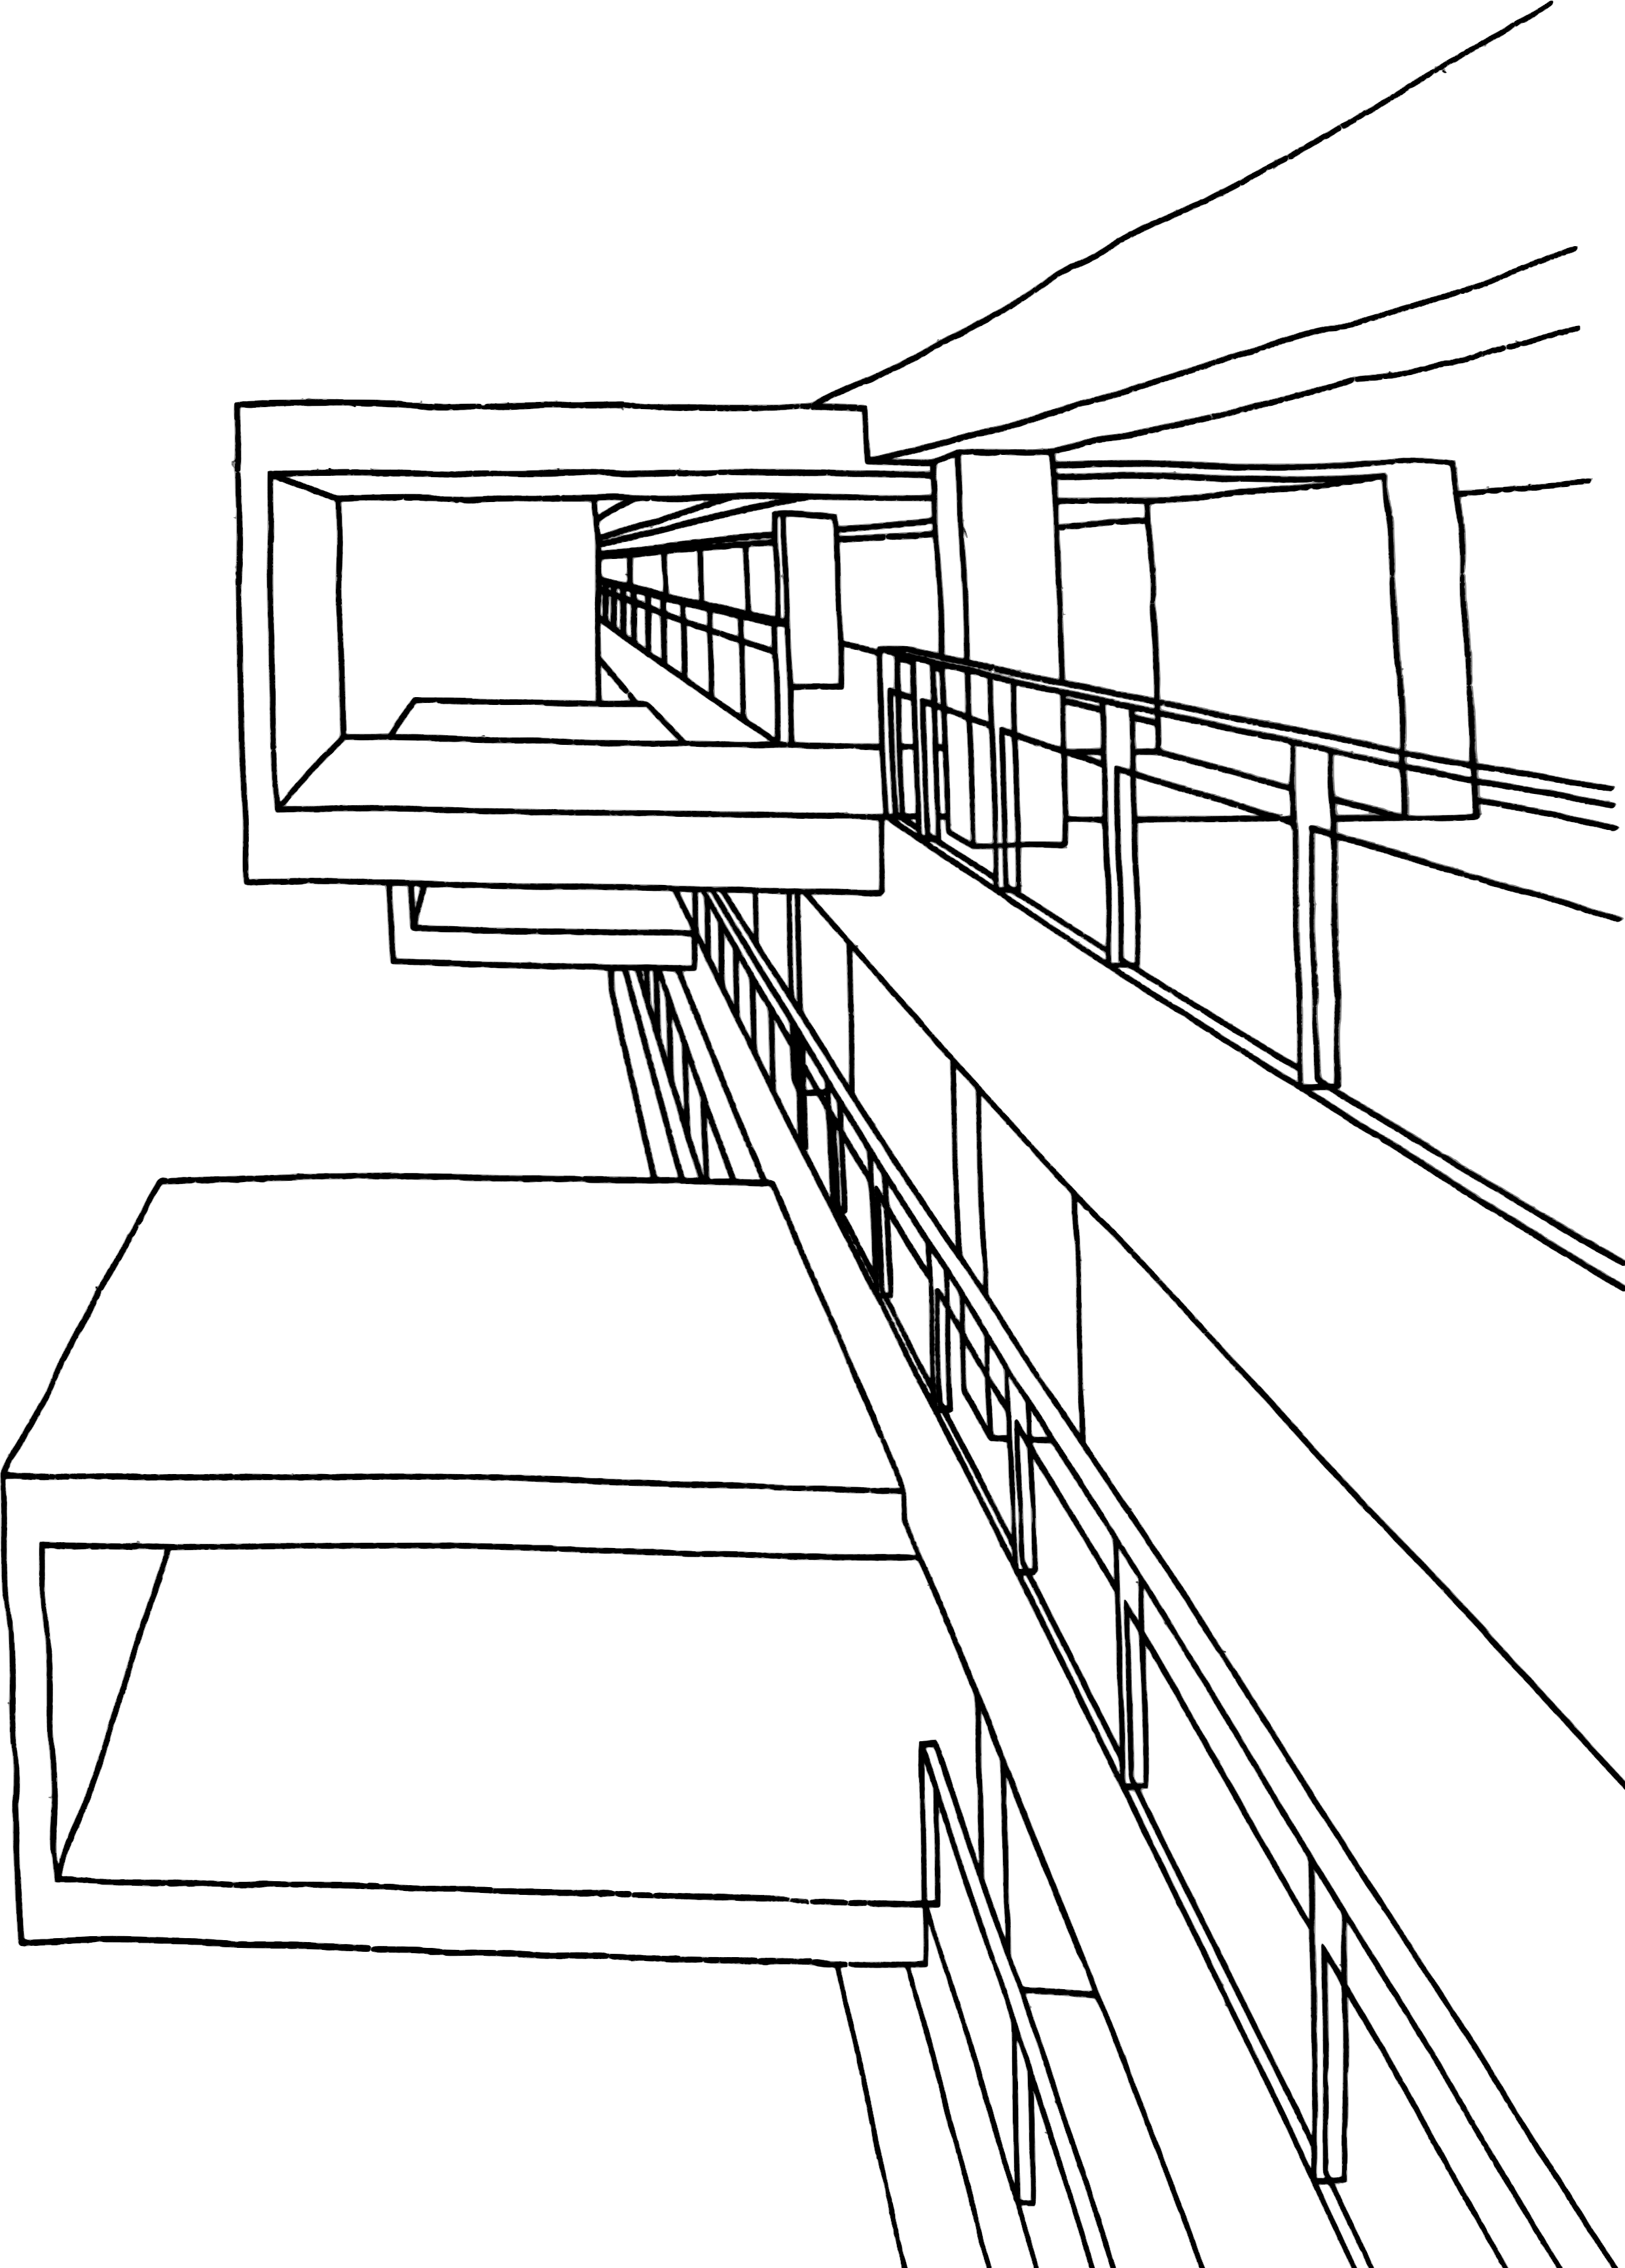
\includegraphics[width=12cm]{images/itu_graphics.png}}
\end{figure}

\restoregeometry


\pagenumbering{arabic}
\section{Introduction}

The following report describes project work done during the course. The first part will go over the system architecture and current status. The process perspective will look into the group's ways of working, and the development of the system. The last part describes important lessons learned, and what the group hopes to bring to future work in the field of DevOps. 
\section{System Perspective}

%A description and illustration of the:

\subsection{System Architecture}
%Design and architecture of your ITU-MiniTwit systems
%Important interactions of subsystems
The following sections will go through various viewpoints to describe the architecture of our system. All views are created in accordance with the UML approach from Christensen et al. \cite{christensen2016_uml}. 

\subsubsection{Module Viewpoint}

Figure \ref{fig:repo-visualized} shows a code visualization of our repository. In this view, generated by Amelia Wattenberger's codebase visualizer \cite{codebase_visualizer}, grey circles represent directories, while filled-in circles represent files, the color corresponding to a file format and its size to the file size. We include this view to give a broad overview of our repository and to give an idea of the size of the different files and directories, which is not possible to show with a package overview diagram. In addition, we point to the fact that the grafana, filebeat, and terraform directories lie outside the main application directory. Note that the \texttt{flag\_tool} directory and several \texttt{.md} files have been omitted from this view. \\

\begin{figure}[]
    \centering
    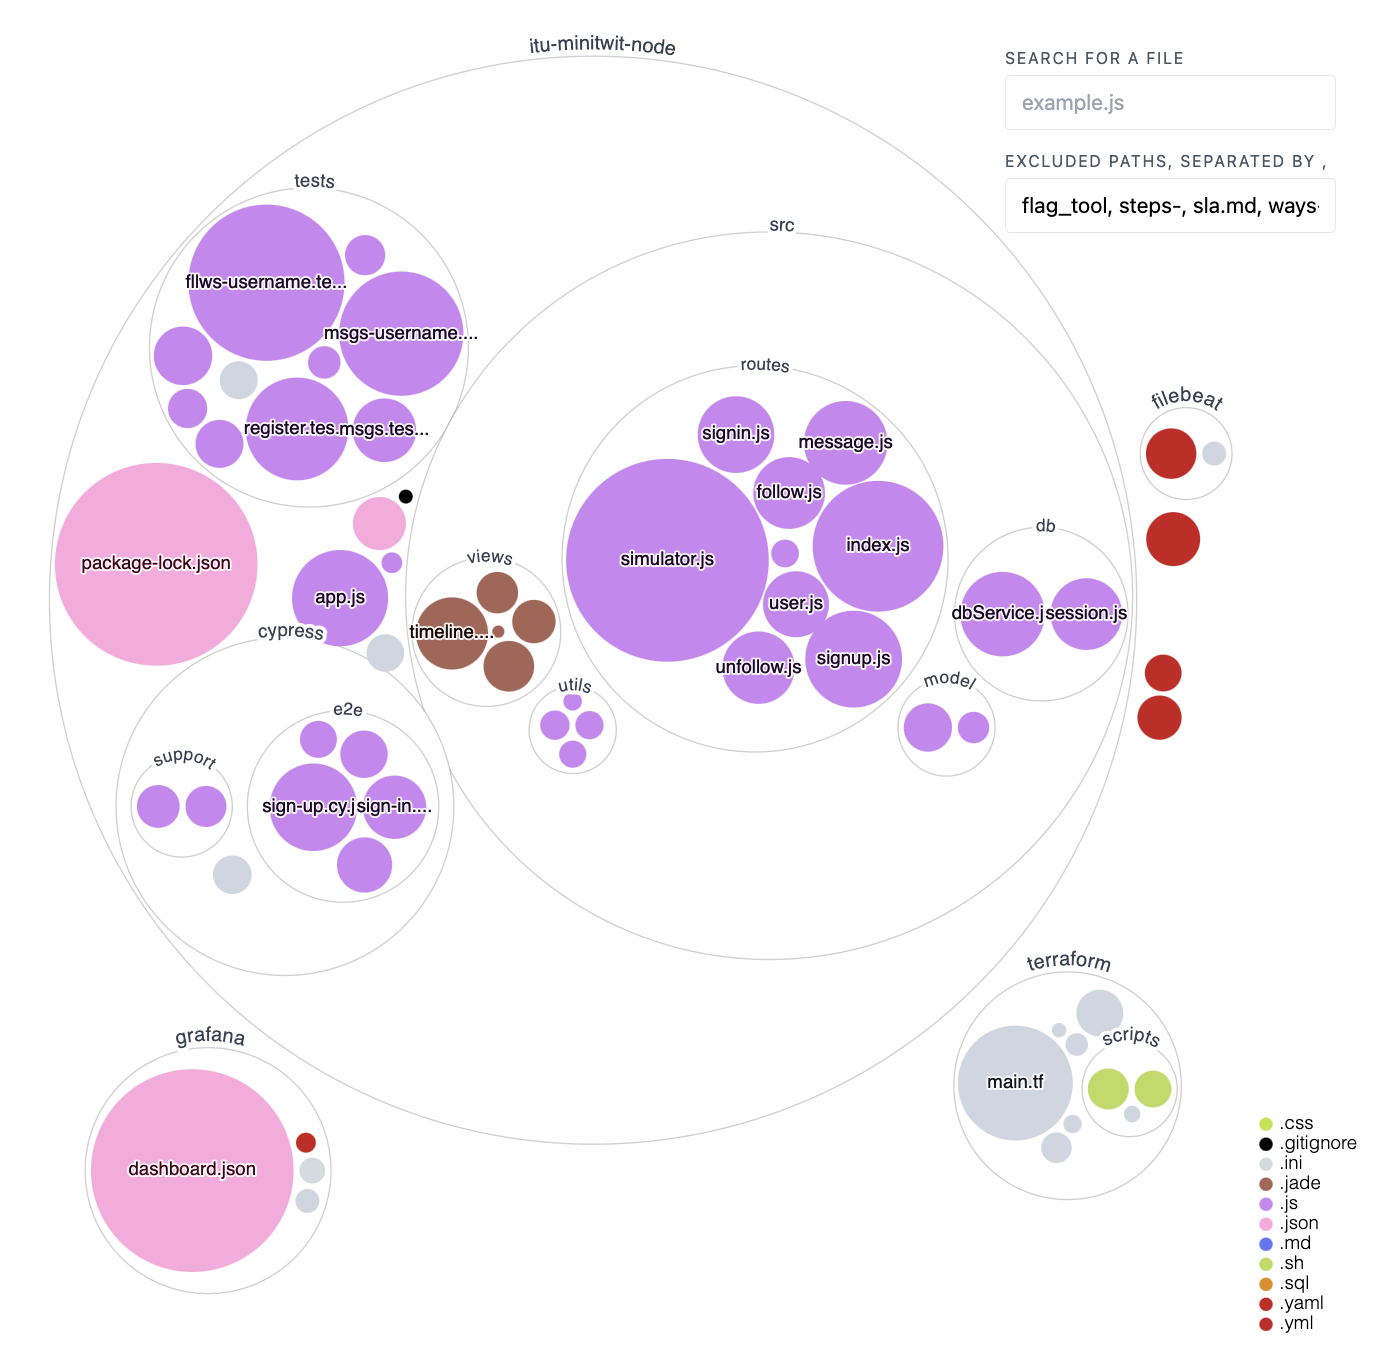
\includegraphics[width=\linewidth]{images/repo-visualizer.png}
    \caption{Visualization of our GitHub repository}
    \label{fig:repo-visualized}
\end{figure}

Figure \ref{fig:module-minitwit} shows a package overview diagram of the web app. Here we observe the dependencies between source files, the test directories, and the main \texttt{app.js} file. If we examine the \texttt{src} directory in more detail, as illustrated in Figure \ref{fig:module-src}, it becomes apparent that the \texttt{routes} directory relies heavily on various other components of the code, as all the app's endpoints are located within this directory. \\

\begin{figure}[H]
    \centering
    \begin{minipage}{0.45\textwidth}
        \centering
        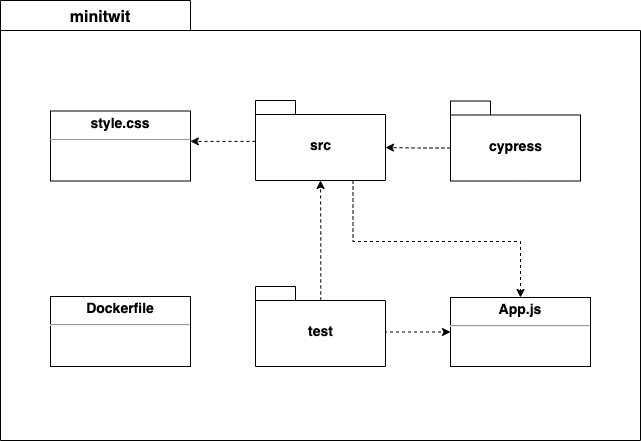
\includegraphics[width=.95\linewidth]{images/module-minitwit.png}
        \caption{Package overview diagram for the \texttt{minitwit} directory}
        \label{fig:module-minitwit}
    \end{minipage}\hfill
    \begin{minipage}{0.45\textwidth}
        \centering
        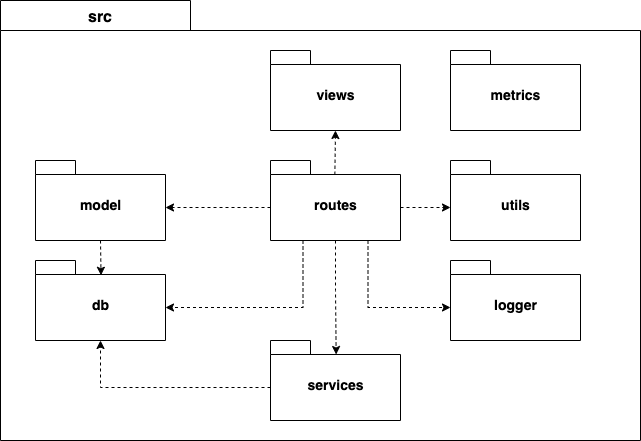
\includegraphics[width=.95\linewidth]{images/module-src.png}
        \caption{Decomposition of the \texttt{src} package}
        \label{fig:module-src}
    \end{minipage}
\end{figure}

\subsubsection{Component and Connector Viewpoint}

The sequence diagram shown in Figure \ref{fig:sequence-login} shows the interaction between subsystems in the scenario where a user successfully logs into the system. Had the username or password been wrong, the error would have been logged instead. \\

\begin{figure}[]
    \centering
    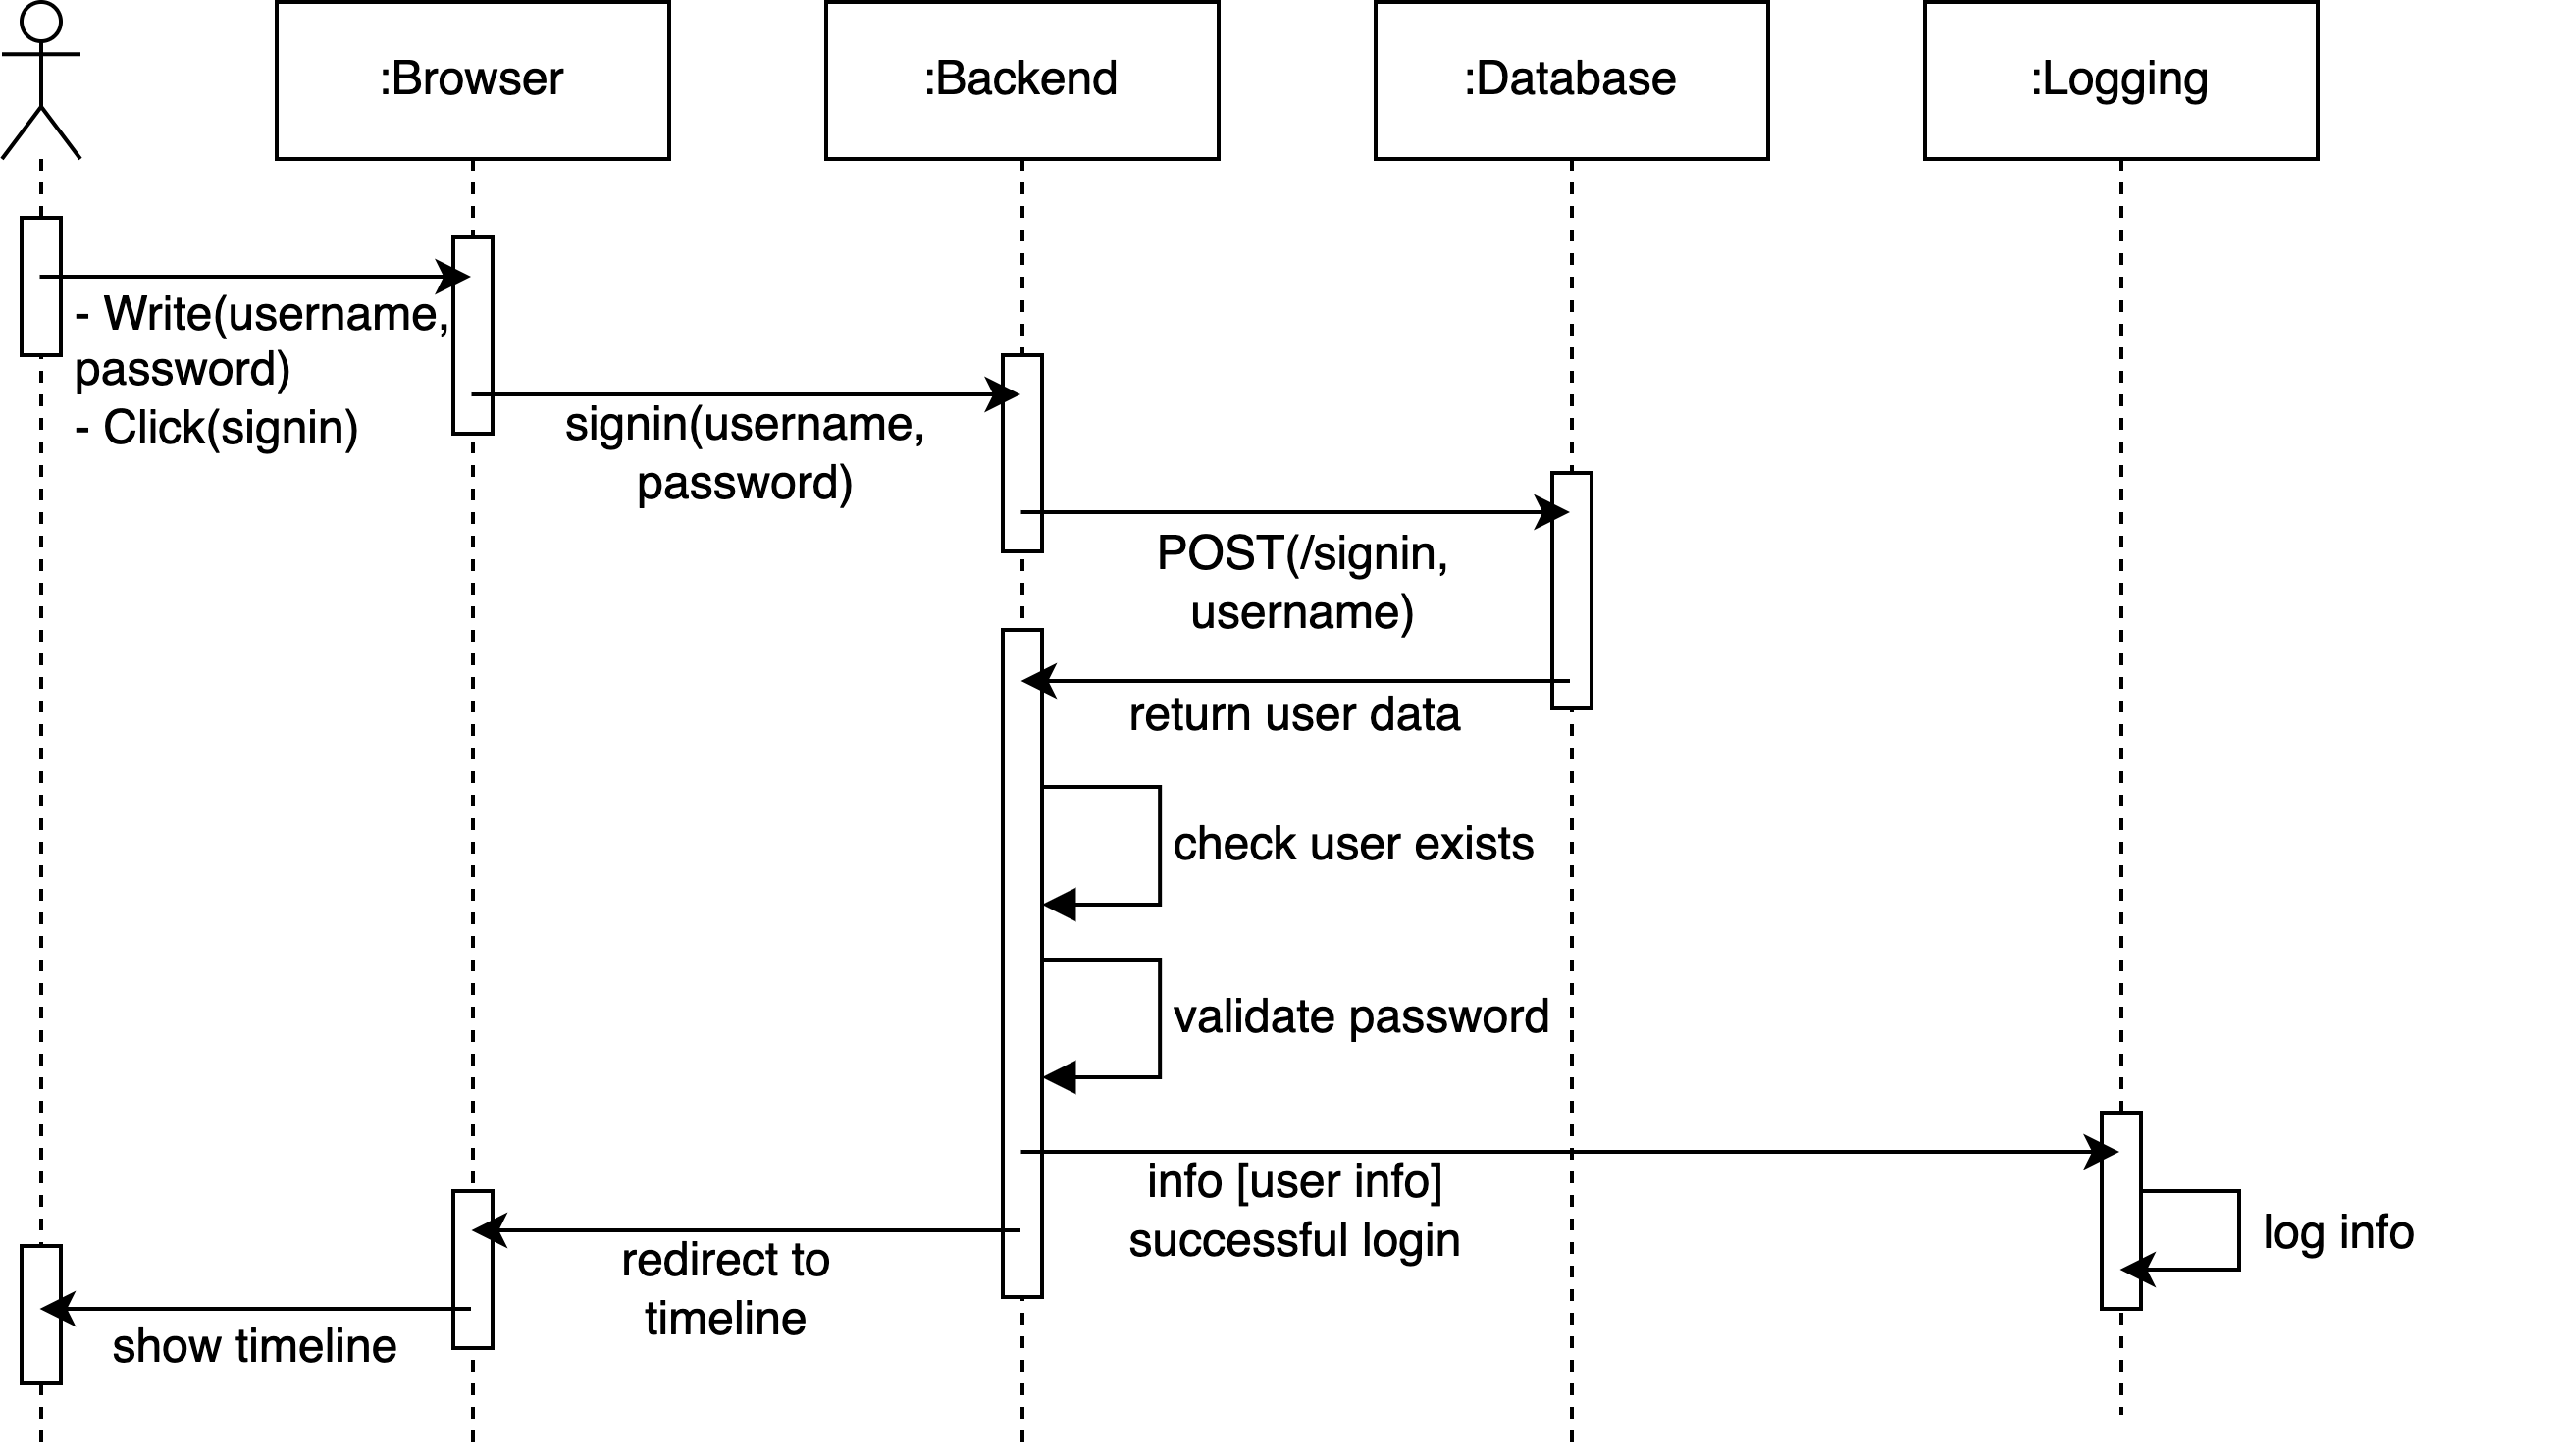
\includegraphics[width=\linewidth]{images/sequence-diagram.png}
    \caption{Sequence diagram of a successful login scenario}
    \label{fig:sequence-login}
\end{figure}

\subsubsection{Allocation Viewpoint}

Figure \ref{fig:deployment-diagram} shows a deployment view of our system. Note that dependencies among software elements have been omitted from this view. This view shows how our software elements are allocated to (virtual) environmental elements at runtime. Software elements in blue can be allocated to any of the environmental elements in red, in accordance with constraints put on our Docker Swarm. The elements in blue are in several layers (ex. the Minitwit component) if specified to be in several replicas.  

% Note that software elements marked in blue can be allocated to 

\begin{figure}[]
    \centering
    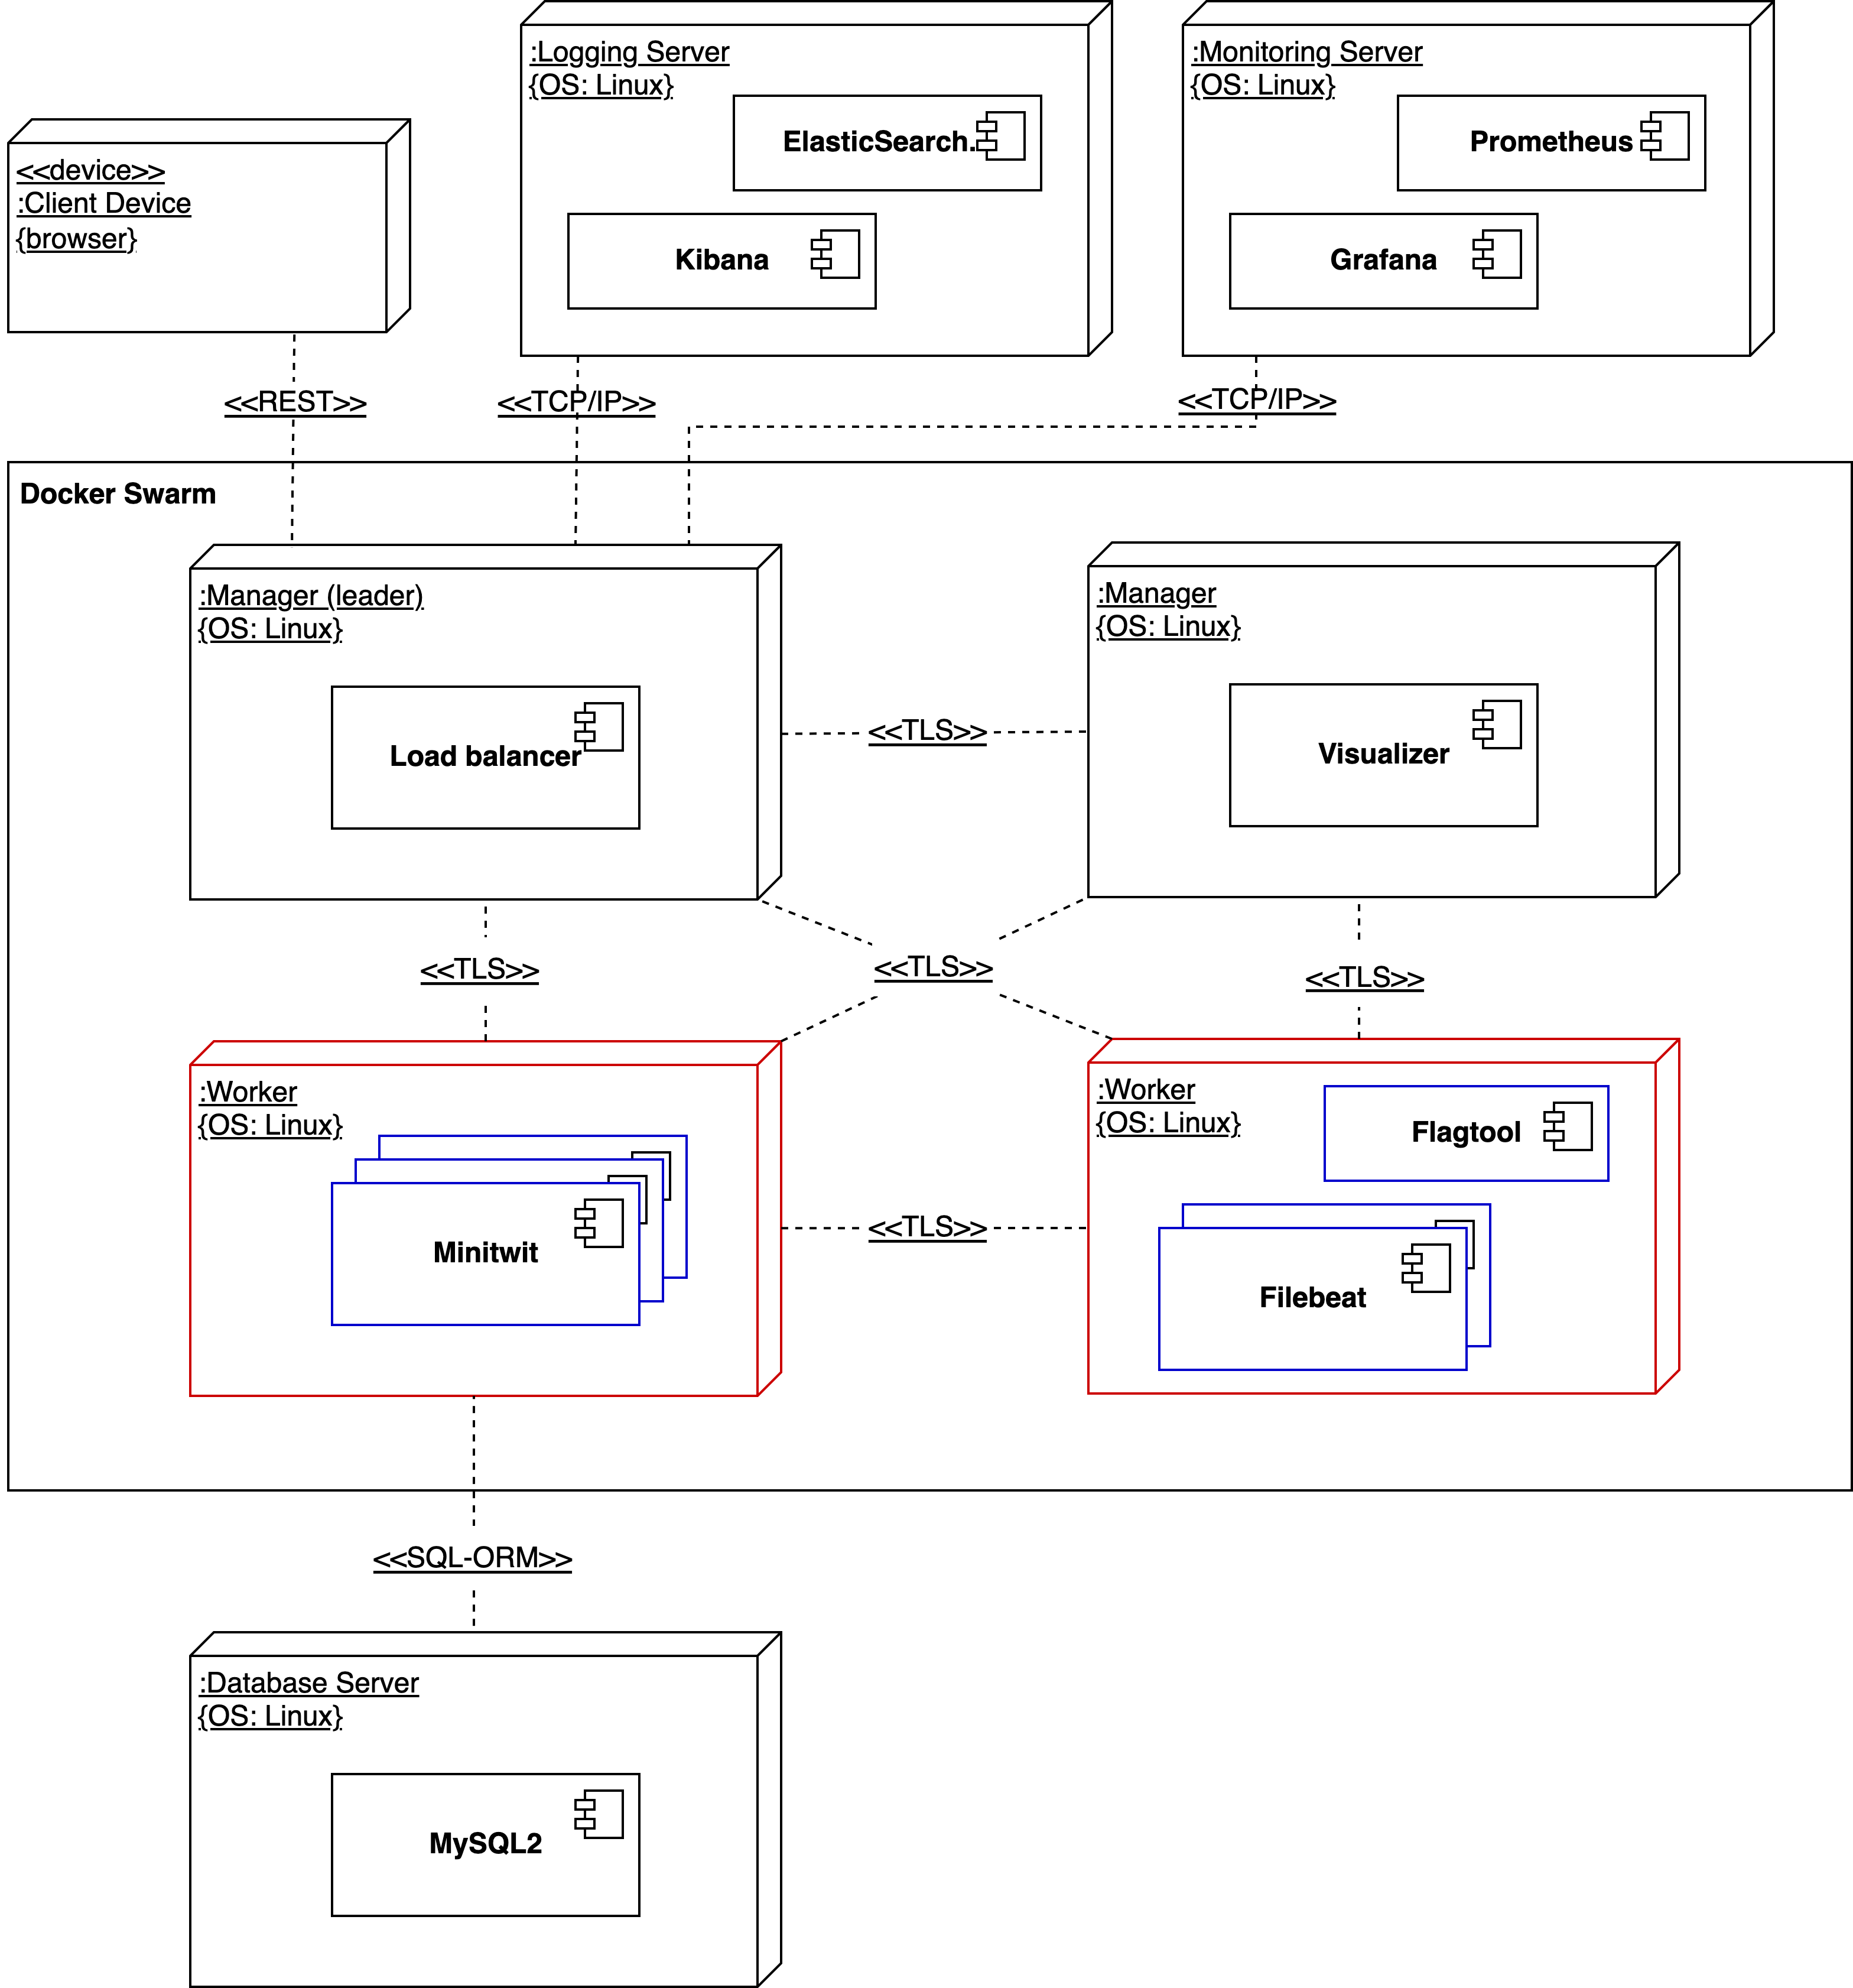
\includegraphics[width=\linewidth]{images/deployment-diagram.png}
    \caption{Deployment diagram of the Minitwit system}
    \label{fig:deployment-diagram}
\end{figure}


\subsection{Arguments for key technology/tool choices}

A list of all dependencies in the system can be found in Appendix \ref{app:dependencies}. \\

% OBS MSc students: Remember to log and provide good arguments for the choice of programming language and framework. Likely, a feature mapping/comparison or a mini-benchmark is a good choice. 

\textbf{Programming language and frameworks}\\
We chose JavaScript, as it is a popular and versatile language for web development that the team wanted to have more experience with. It also allows for a wide selection of front-end frameworks. We used the Pug library, allowing us to get started quickly and efficiently. While we initially considered transitioning to Vue.js or another modern framework for enhanced functionality, time constraints compelled us to prioritize the completion of mandatory assignments.\\ 

% OBS MSc students: Remember to log and provide good arguments for the choice of virtualization techniques and deployment targets 

\textbf{Virtualization technique and deployment targets}\\
We chose the containerization virtualization technique with cloud deployment. Containerization was chosen because of the apparent values it brings, such as being portable, ensuring that the application can run consistently in any environment, and being agile, since it is fast and easy to create, deploy, and destroy containers. We chose cloud deployment since none of the group members had the required setup for on-premise hosting and because of the convenience it brings, such as handling scaling and reduced infrastructure management. After shortly considering other opportunities, we selected DigitalOcean as our deployment platform, as suggested in the course.Among the most important benefits of the platform, we found an intuitive user experience and a 200 dollars credit included in accounts for academical purposes.
\\

% OBS MSc students: Remember to log and provide good arguments for the choice of ORM framework and chosen DBMS

\textbf{DBMS and ORM framework}\\
We opted to use MySQL as our chosen DBMS because it employs a relational data model, organizing data into tables and enforcing a fixed scheme. This structure aligns well with our application's needs, as it has a limited and well-defined set of data types. While PostgreSQL also supports this need and offers comparable features, the decision between MySQL and PostgreSQL was somewhat arbitrary due to their similar capabilities in this regard. As our ORM framework, we used Sequelize as it is widely used with Node.js applications and offers a comprehensive set of features for working with databases. Although it was compelling to try a self-hosted database to learn how to deal with infrastructure management, maintenance, backups, and disaster recovery planning, we decided to go with a hosted database option provided by DigitalOcean for its convenience and ease of use.

\subsection{Current state of the system}
%Describe the current state of your systems, for example using results of static analysis and quality assessments.

All the applications are fully functional. However, the system is currently shut down due to a lack of credits in DigitalOcean. We use SonarCloud as our quality management platform which runs automatic checks of our code after each pushed change. It detects potential vulnerabilities, bugs, code smells, and code duplication. Our codebase contains a significant number of code smells, primarily because our main focus was on addressing bugs and vulnerabilities rather than prioritizing their removal. Below, you can find a dashboard of the latest analysis in Figure \ref{fig:sonarCloud}. 

\begin{figure}[H]
    \centering
    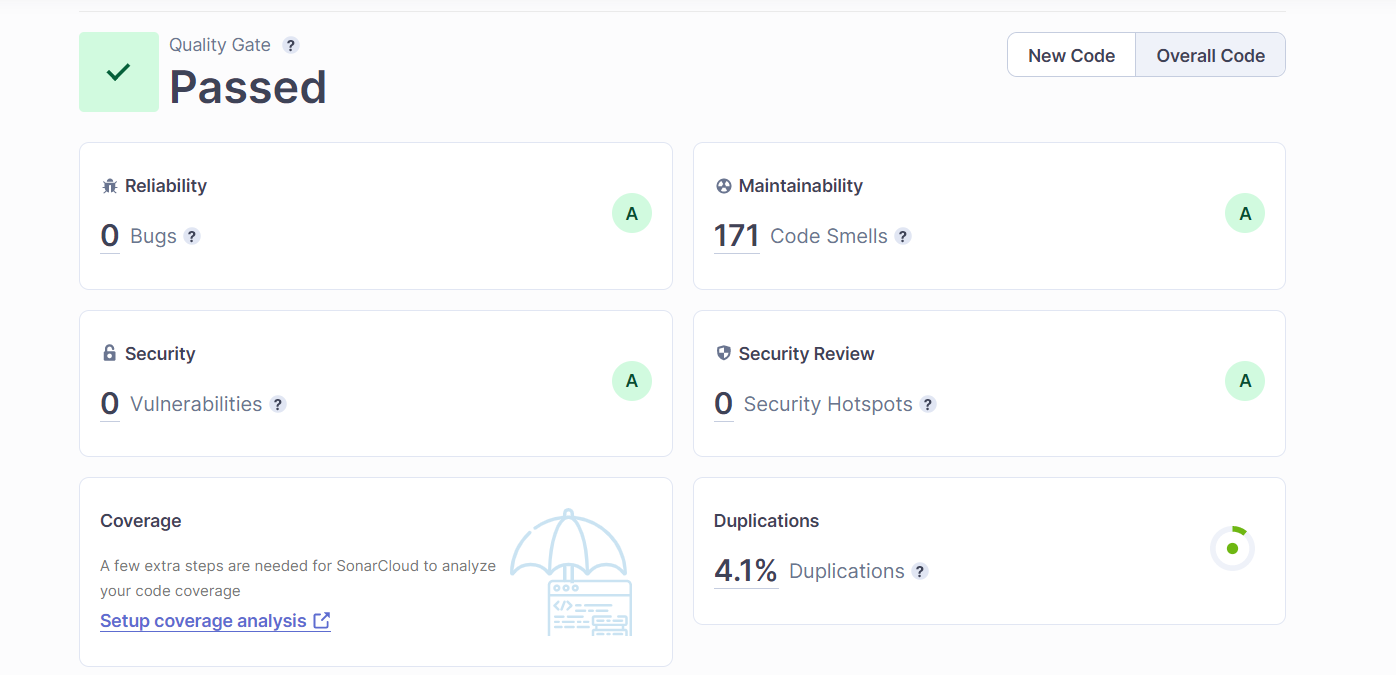
\includegraphics[width=\linewidth]{images/SonarCloud.png}
    \caption{SonarCloud analysis of our repository.}
    \label{fig:sonarCloud}
\end{figure}

\subsection{License}
We have chosen an MIT license since we using Node.js and npm packages are overwhelmingly using the MIT license or similar licenses \cite{choosealicense}. The license is added in our \texttt{root} folder. 

%Finally, describe briefly, if the license that you have chosen for your project is actually compatible with the licenses of all your direct dependencies.


% REMEMBER THE FOLLOWING:

%Double check that for all the weekly tasks (those listed in the schedule) you include the corresponding information.

%MSc students remember to argue for the choice of technologies and decisions for at least all cases for which we asked you to do so in the tasks at the end of each session.


\section{Process Perspective}

%A description and illustration of:

\subsection{Team work}

%How do you interact as developers? 
%How is the team organized?
%Applied development process and tools supporting it
%For example, how did you use issues, Kanban boards, etc. to organize open tasks
%Applied branching strategy.

\subsubsection{Team organization}

Our project group has embraced a Scrum-like approach, working without a designated leader or specific areas of responsibility. We have integrated various elements from the Scrum framework into our week-to-week project work. We have prioritized meeting physically and working together, and have done so twice a week. During these meetings, we have conducted daily stand-up sessions to discuss progress, align our activities, and coordinate tasks. The remaining time was dedicated to project work, where team members collaborated either in pairs or individually. This flexible approach allowed us to adapt our working arrangements based on the tasks at hand and the preferences of team members.

\subsubsection{Collaboration and communication tools}

We have used \textit{Microsoft Teams} as the primary channel of day-to-day online communication. In addition, we used \textit{Notion} as a shared space for note-taking and organizing links to relevant resources, see Figure \ref{fig:notion}. 

\begin{figure}[H]
    \centering
    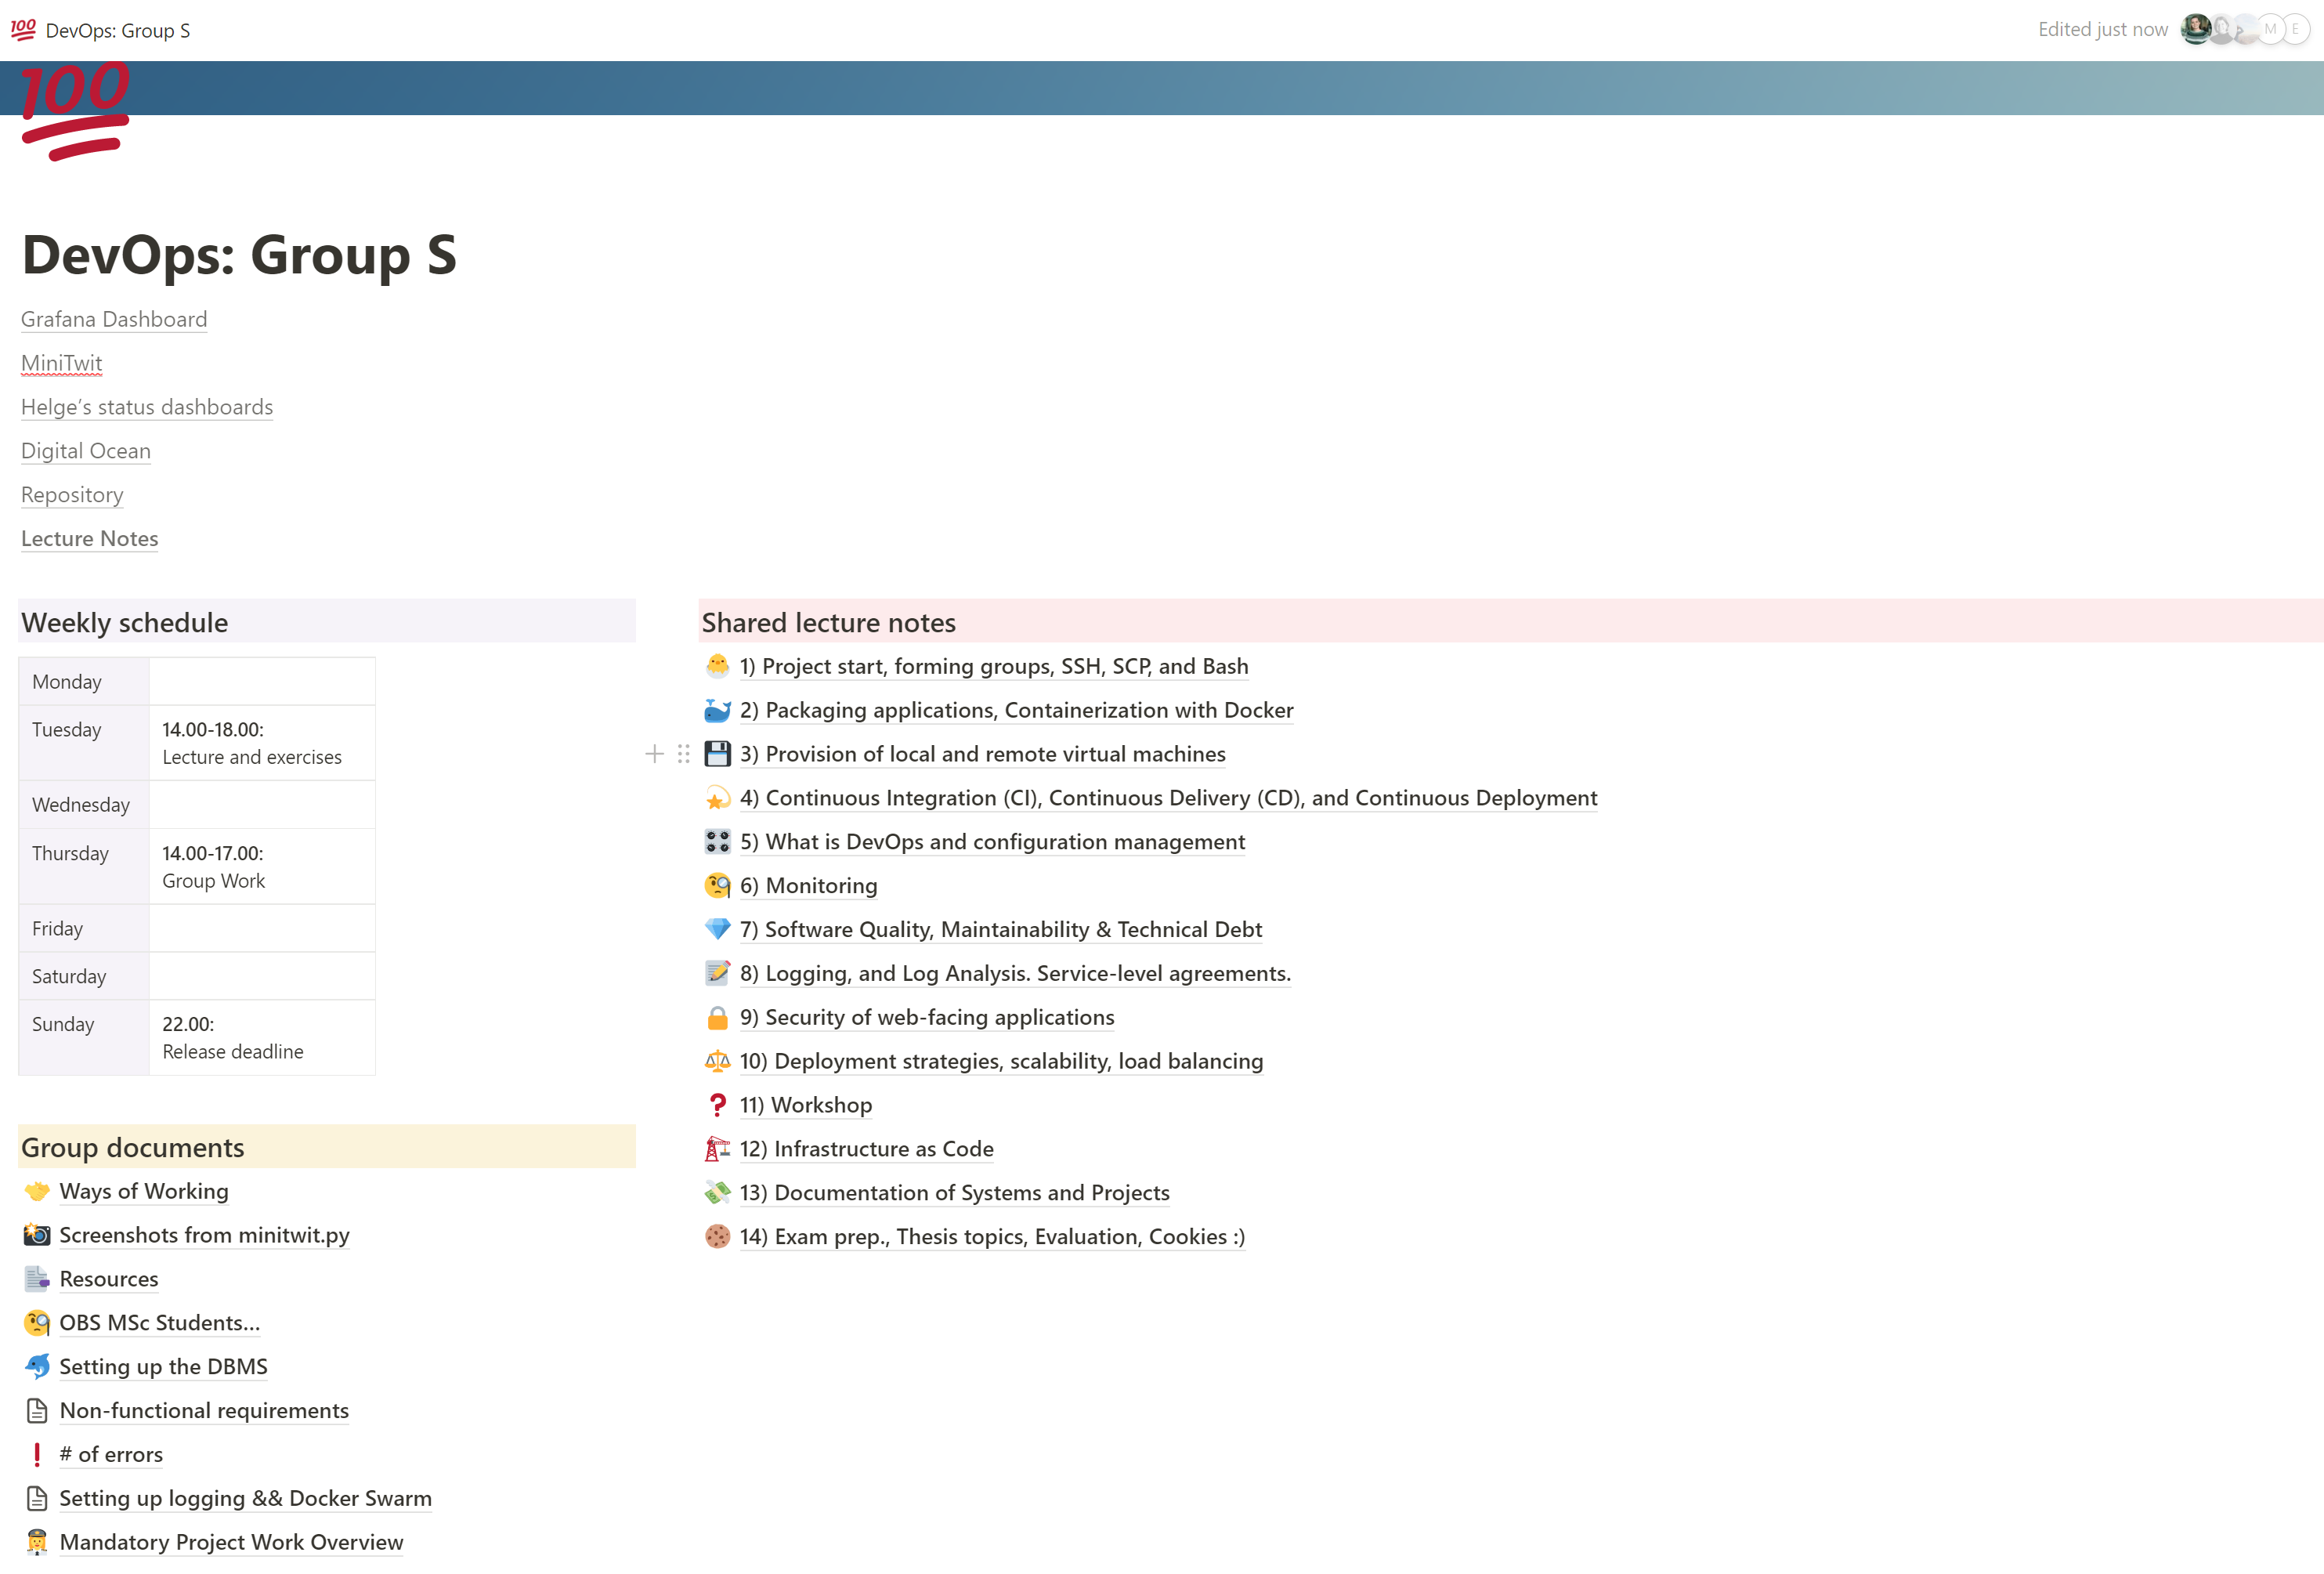
\includegraphics[width=.85\linewidth]{images/notion.png}
    \caption{Shared Notion.}
    \label{fig:notion}
\end{figure}

In addition to storing our MiniTwit repository, which will be further explained in the next section, we also used \textit{Github} for organizing tasks. Every Tuesday, following the lecture, we divided the tasks for the current week into subtasks on a Kanban board in our GitHub project and prioritized the new tasks in comparison to uncompleted tasks from the previous weeks. The board was consistently updated throughout the project with new task assignments and overall task progress, see Figure \ref{fig:kanban}. We used the Backlog-column for every unprioritized task, and the Todo column for the prioritized task the given week. 

\begin{figure}[H]
    \centering
    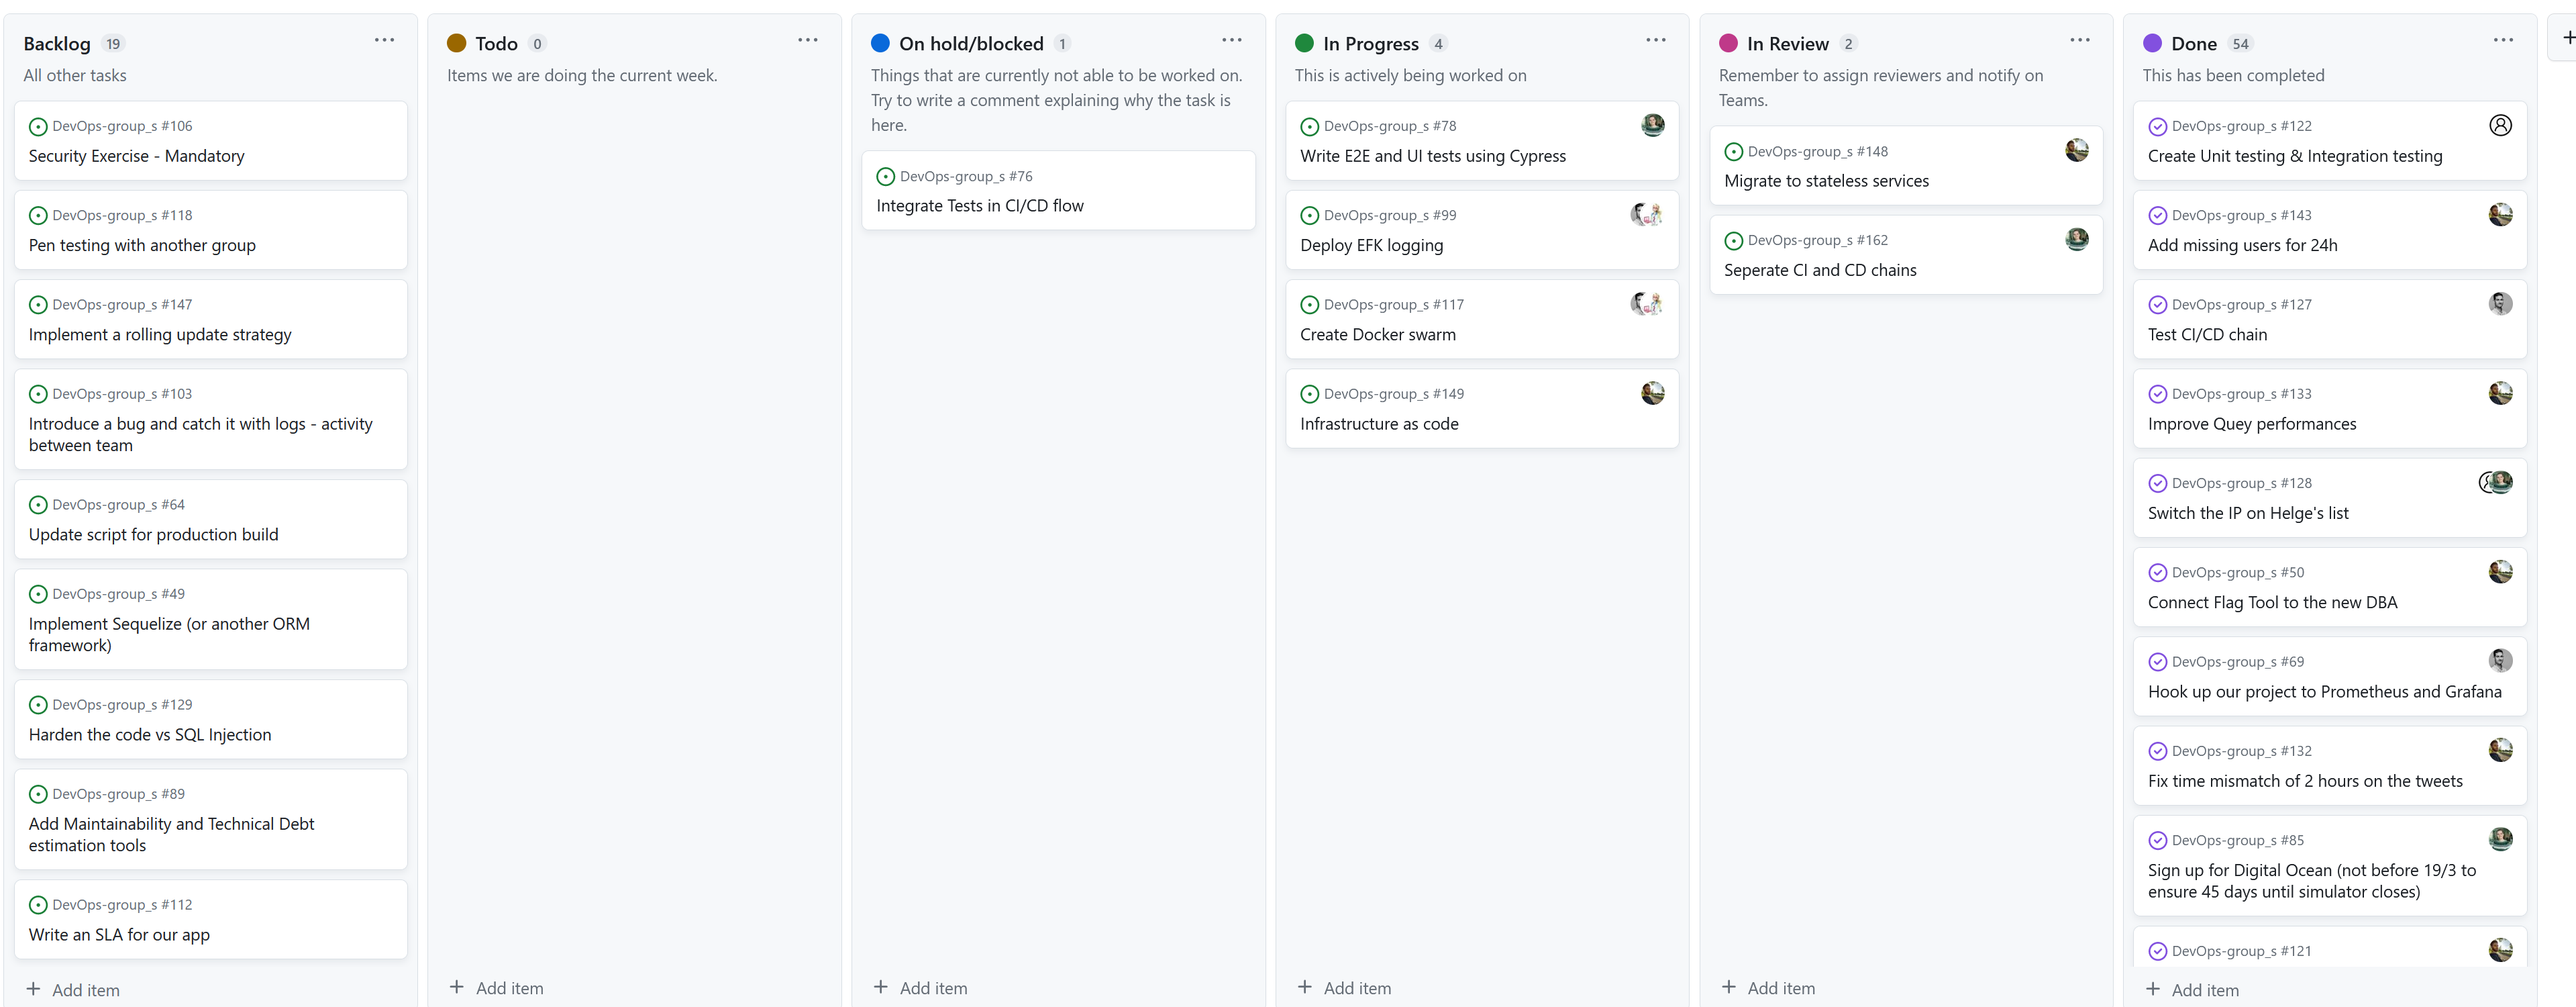
\includegraphics[width=\linewidth]{images/kanban.png}
    \caption{Our Kanban board}
    \label{fig:kanban}
\end{figure}

\subsubsection{Branching strategy}

Our team has implemented the Github Flow \cite{github_flow} branching strategy, which has one central \texttt{main} branch. To add new features, we start by checking out the \texttt{main} branch and push working changes to this local feature branch. Once the development work is completed, we create a pull request. Each pull request undergoes checks for merge conflicts, triggers our continuous integration (CI) pipeline, and requires review by at least one other team member.\\

The primary benefit of this approach lies in its simplicity. However, it also requires thorough checking and testing since it relies on a single central main branch. Our experience with this approach has highlighted certain challenges. Specifically, since we only added tests and separated our CI/CD chains relatively late in the process, we encountered issues with having to roll back \texttt{main}. This was due to only operating with a continuous deployment configuration which was triggered when changes were pushed to \texttt{main}.  

\subsection{CI/CD chains} 

%A complete description of stages and tools included in the CI/CD chains.
%That is, including deployment and release of your systems.

% OBS MSc students: Remember to log and provide good arguments for the choice of CI/CD system, i.e., why do you choose your solution instead of any other?

\subsubsection{Continuous Integration}

Our CI chain, see Figure \ref{fig:ci}, is triggered when a pull request is created. Note that the cypress testing step is grayed out since it was not thoroughly tested in the CI chain before we suspended our application. The diamond shapes are added to indicate where the chain can stop if a step fails. We intend to test and integrate this properly before the exam.\\ 

\noindent The CI chain has four main functionalities:

\begin{enumerate}
    \item Check out code 
    \item Login to Docker Hub
    \item Test the application
    \item Build and push images
\end{enumerate}

Due to time prioritization, we were unable to incorporate static checks into our CI chain. However, if we had implemented static checks, such as code analysis and linters, they would have been included before testing our application. By integrating these checks before testing, we avoid running unnecessary testing on an application that would fail either way. The same principle is the reasoning behind having testing before building and pushing our images.

% to edit: https://app.diagrams.net/#G1GlXy0XzENH587gelZ-4iOpl59S6CnzSF
\begin{figure}[H]
    \centering
    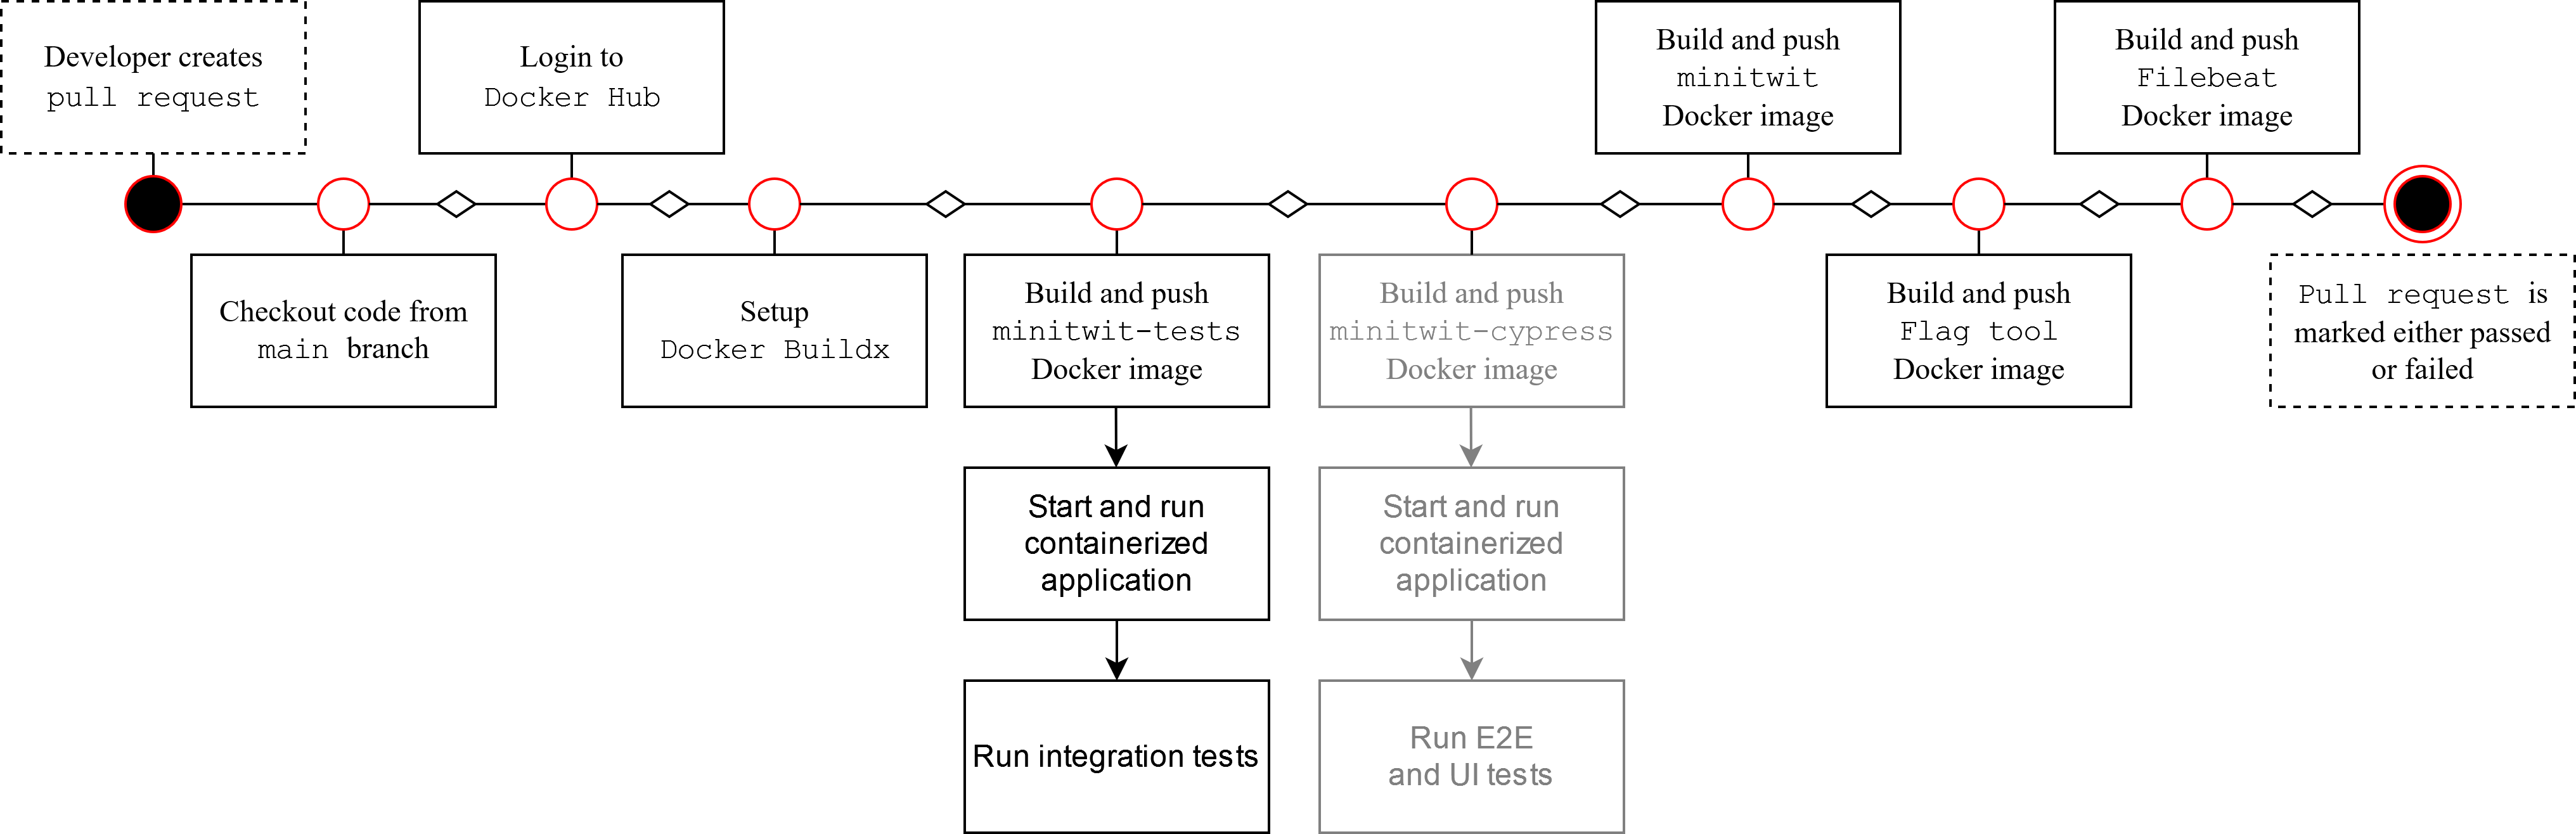
\includegraphics[width=\linewidth]{images/ci-flow.png} 
    \caption{Continous Integration flow diagram.}
    \label{fig:ci}
\end{figure}

In summary, our approach is to complete all necessary steps before deploying the code to our DigitalOcean servers. As part of our CI chain, we have chosen to include the creation and pushing of Docker images instead of placing them in the CD chain. Although these steps often belong in the CD chain, this decision allows us to proactively identify any issues associated with building or packaging the application into Docker images before merging to the main branch. Having limited experience working with Docker images, this approach favours a thorough understanding of Docker systems and documentation in case any issue arise within the images.

\subsubsection{Continuous Deployment}

\noindent Our CD chain, see figure \ref{fig:cd}, has two responsibilities: 

\begin{enumerate}
    \item Making the SSH connection available as an environment variable for the subsequent step in the deployment process
    \item Establishing an SSH connection to the remote server and executing the \texttt{deploy.sh} script
\end{enumerate}

% to edit: https://app.diagrams.net/#G1GlXy0XzENH587gelZ-4iOpl59S6CnzSF (see different tabs) 
\begin{figure}[H]
    \centering
    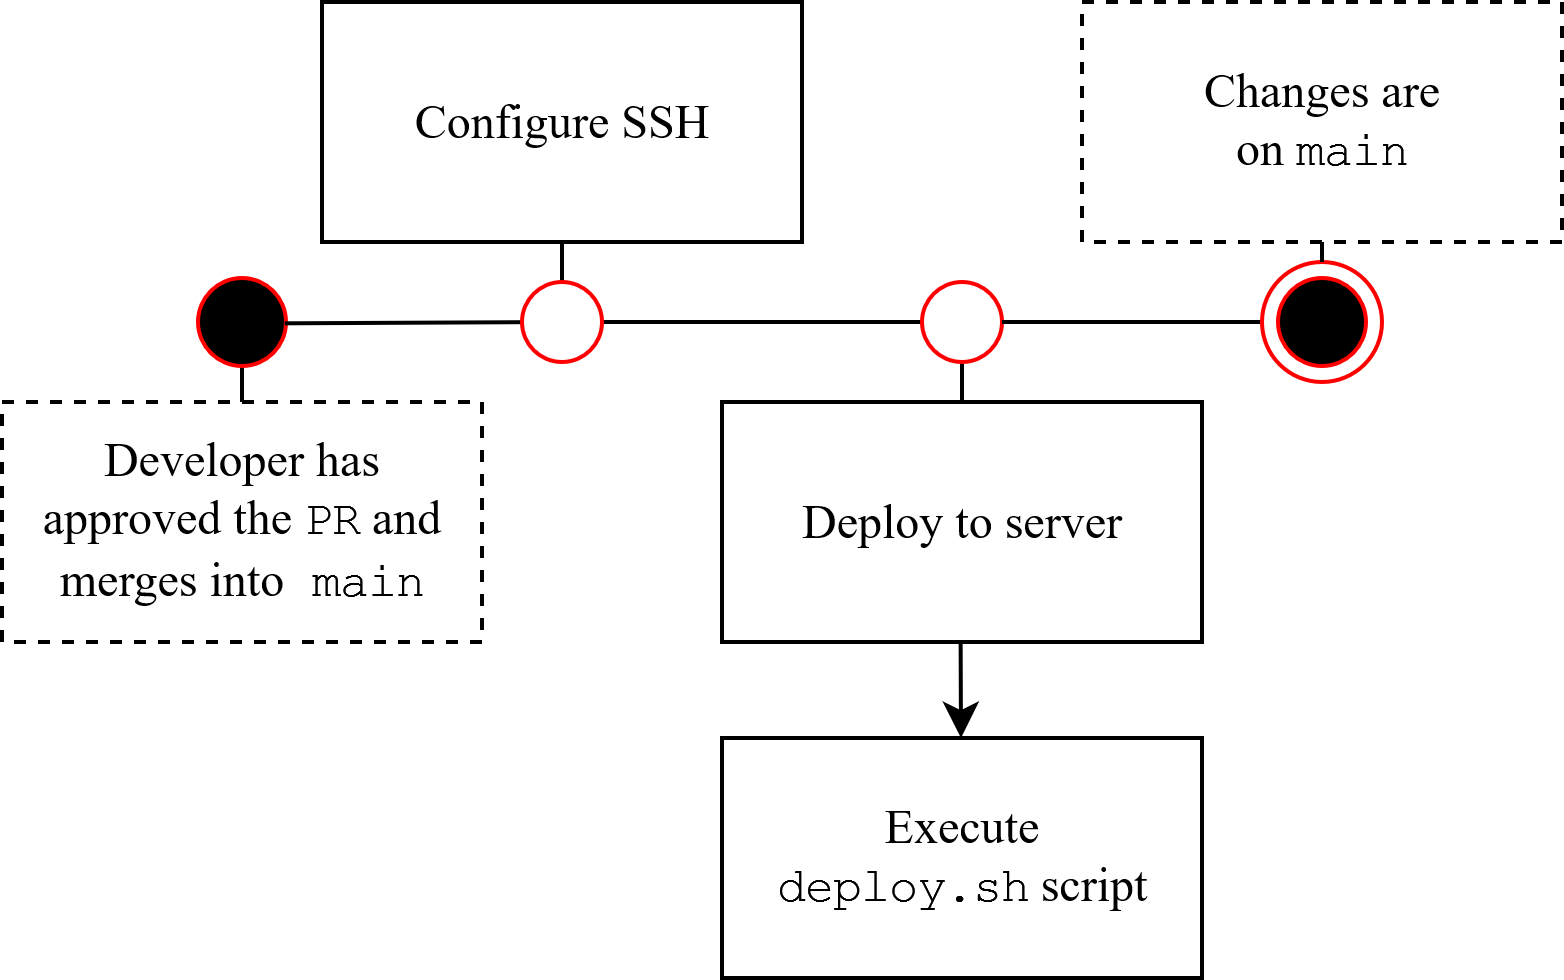
\includegraphics[width=.35\linewidth]{images/cd-flow.png} 
    \caption{Continous Deployment flow diagram.}
    \label{fig:cd}
\end{figure}

We did not manage to implement continuous delivery in the form of automatic releases or rolling updates in our CD chain.\\

When we fully implement using Terraform and enforce infrastructure-as-code, our CD chain will be deprecated. Instead of connecting to our CI/CD droplet and executing the deploy script, we will connect to our DO account via their API. Once connected, Terraform will take the lead in provisioning the resources specified in our repository configuration files. This includes creating or removing VMs, networks, IPs, and other defined components.

\subsection{Repository setup}

%Organization of your repositor(ies).
%That is, either the structure of mono-repository or organization of artifacts across repositories.
%In essence, it has to be clear what is stored where and why.

We chose a mono-repository setup containing the whole project. In the root folder, we have all relevant configuration files as well as sub-folders for every aspect of the system: the application source code, monitoring, and CI/CD pipeline. 

\begin{figure}[H]
    \centering
    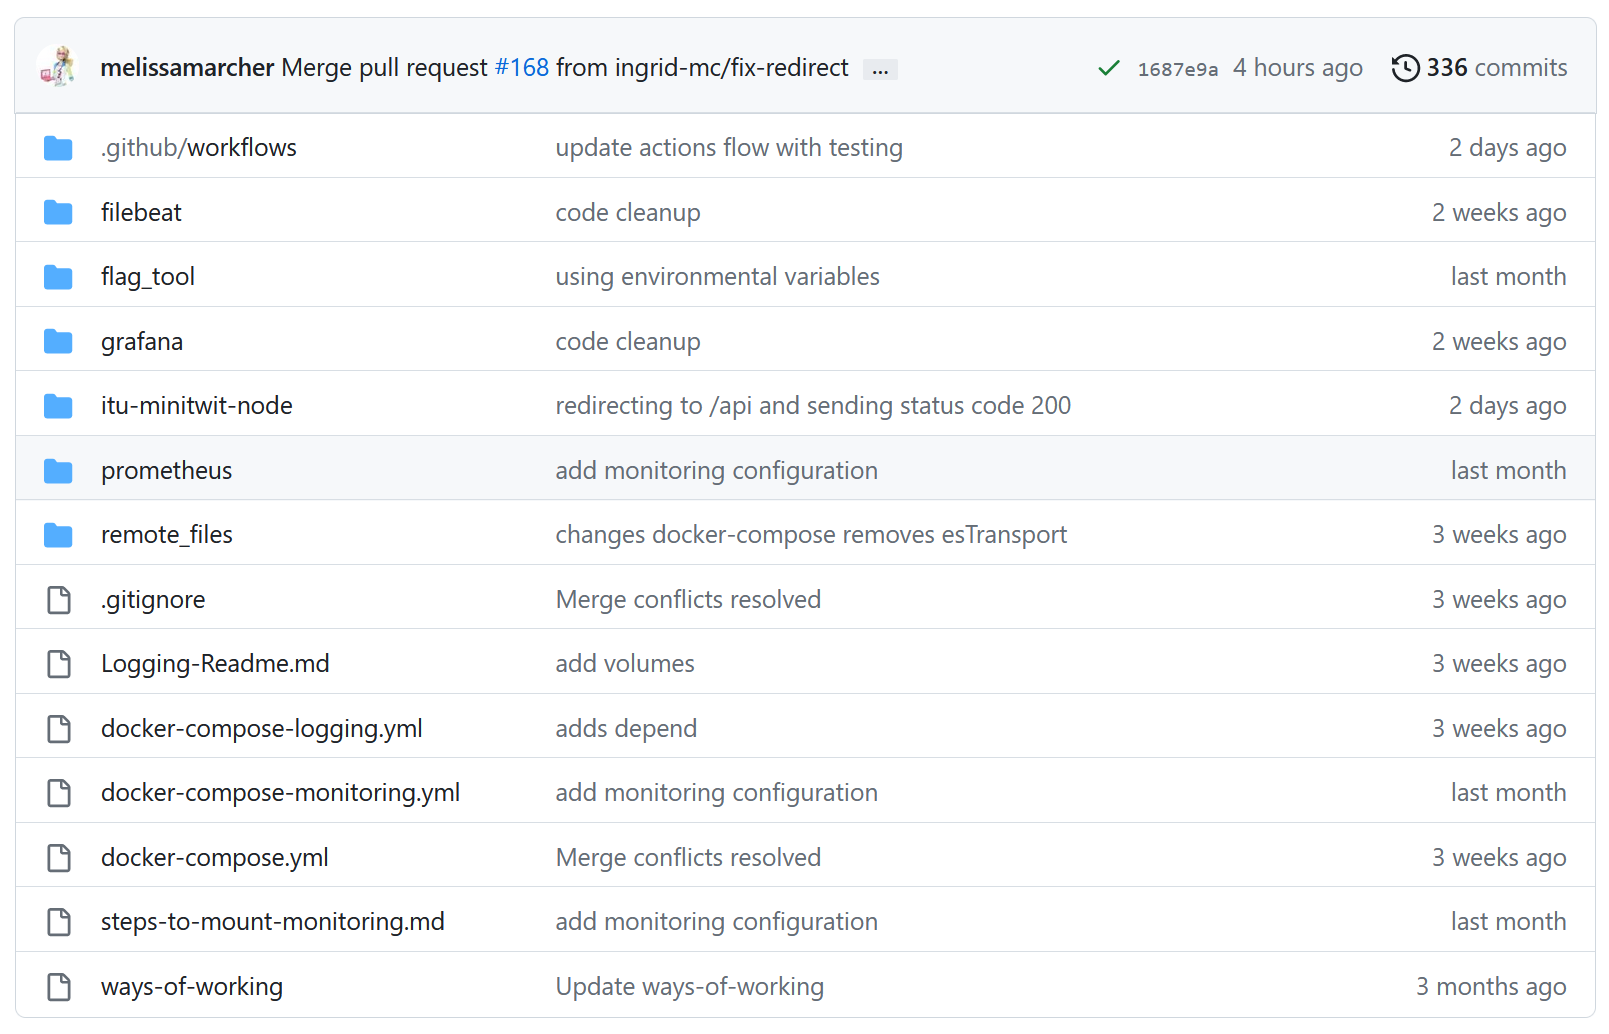
\includegraphics[width=.85\linewidth]{images/repo.png}
    \caption{\texttt{root} folder in our repository}
    \label{fig:repo}
\end{figure}

In the \texttt{itu-minitwit-node} folder, see Figure \ref{fig:minitwit-node}, we have our source code, tests, and Docker files. The \texttt{src} folder is further split into relevant subsystems such as database and entity handling, frontend in \texttt{views}, and routing between pages, see Figure \ref{fig:src} for a full overview.   

\begin{figure}[H]
    \centering
    \begin{minipage}{0.45\textwidth}
        \centering
        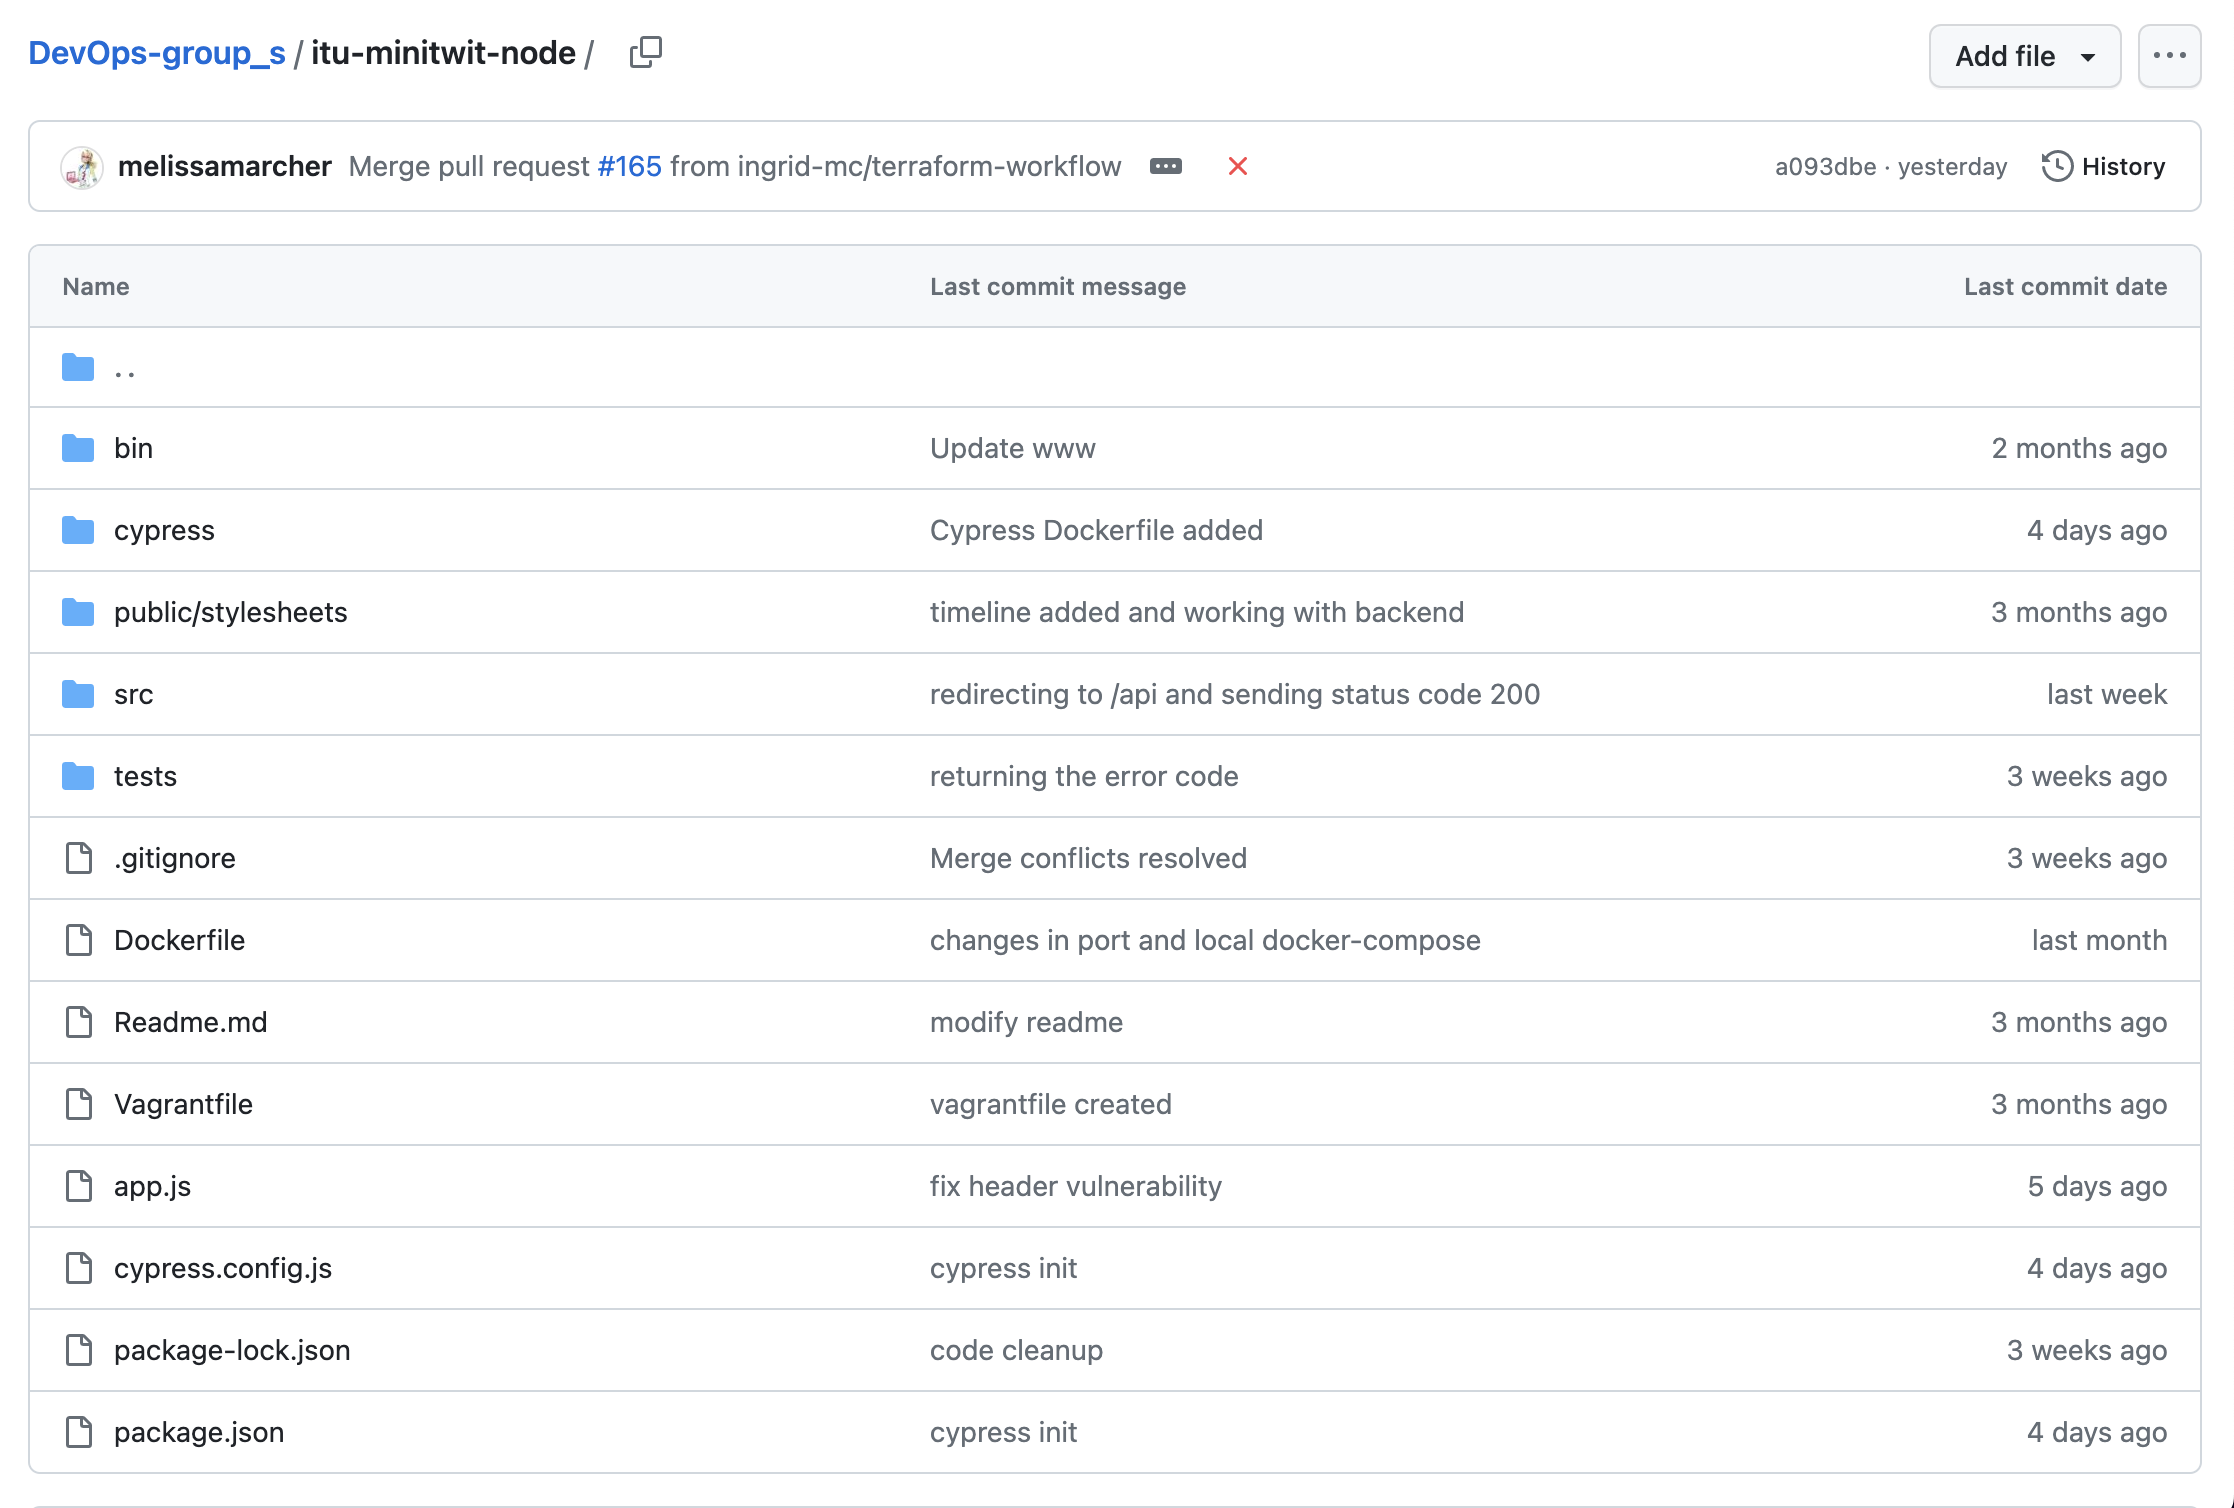
\includegraphics[width=1.15\textwidth]{images/itu-minitwit-node-folder.png}
        \caption{\texttt{itu-minitwit-node} folder}
        \label{fig:minitwit-node}
    \end{minipage}\hfill
    \begin{minipage}{0.45\textwidth}
        \centering
        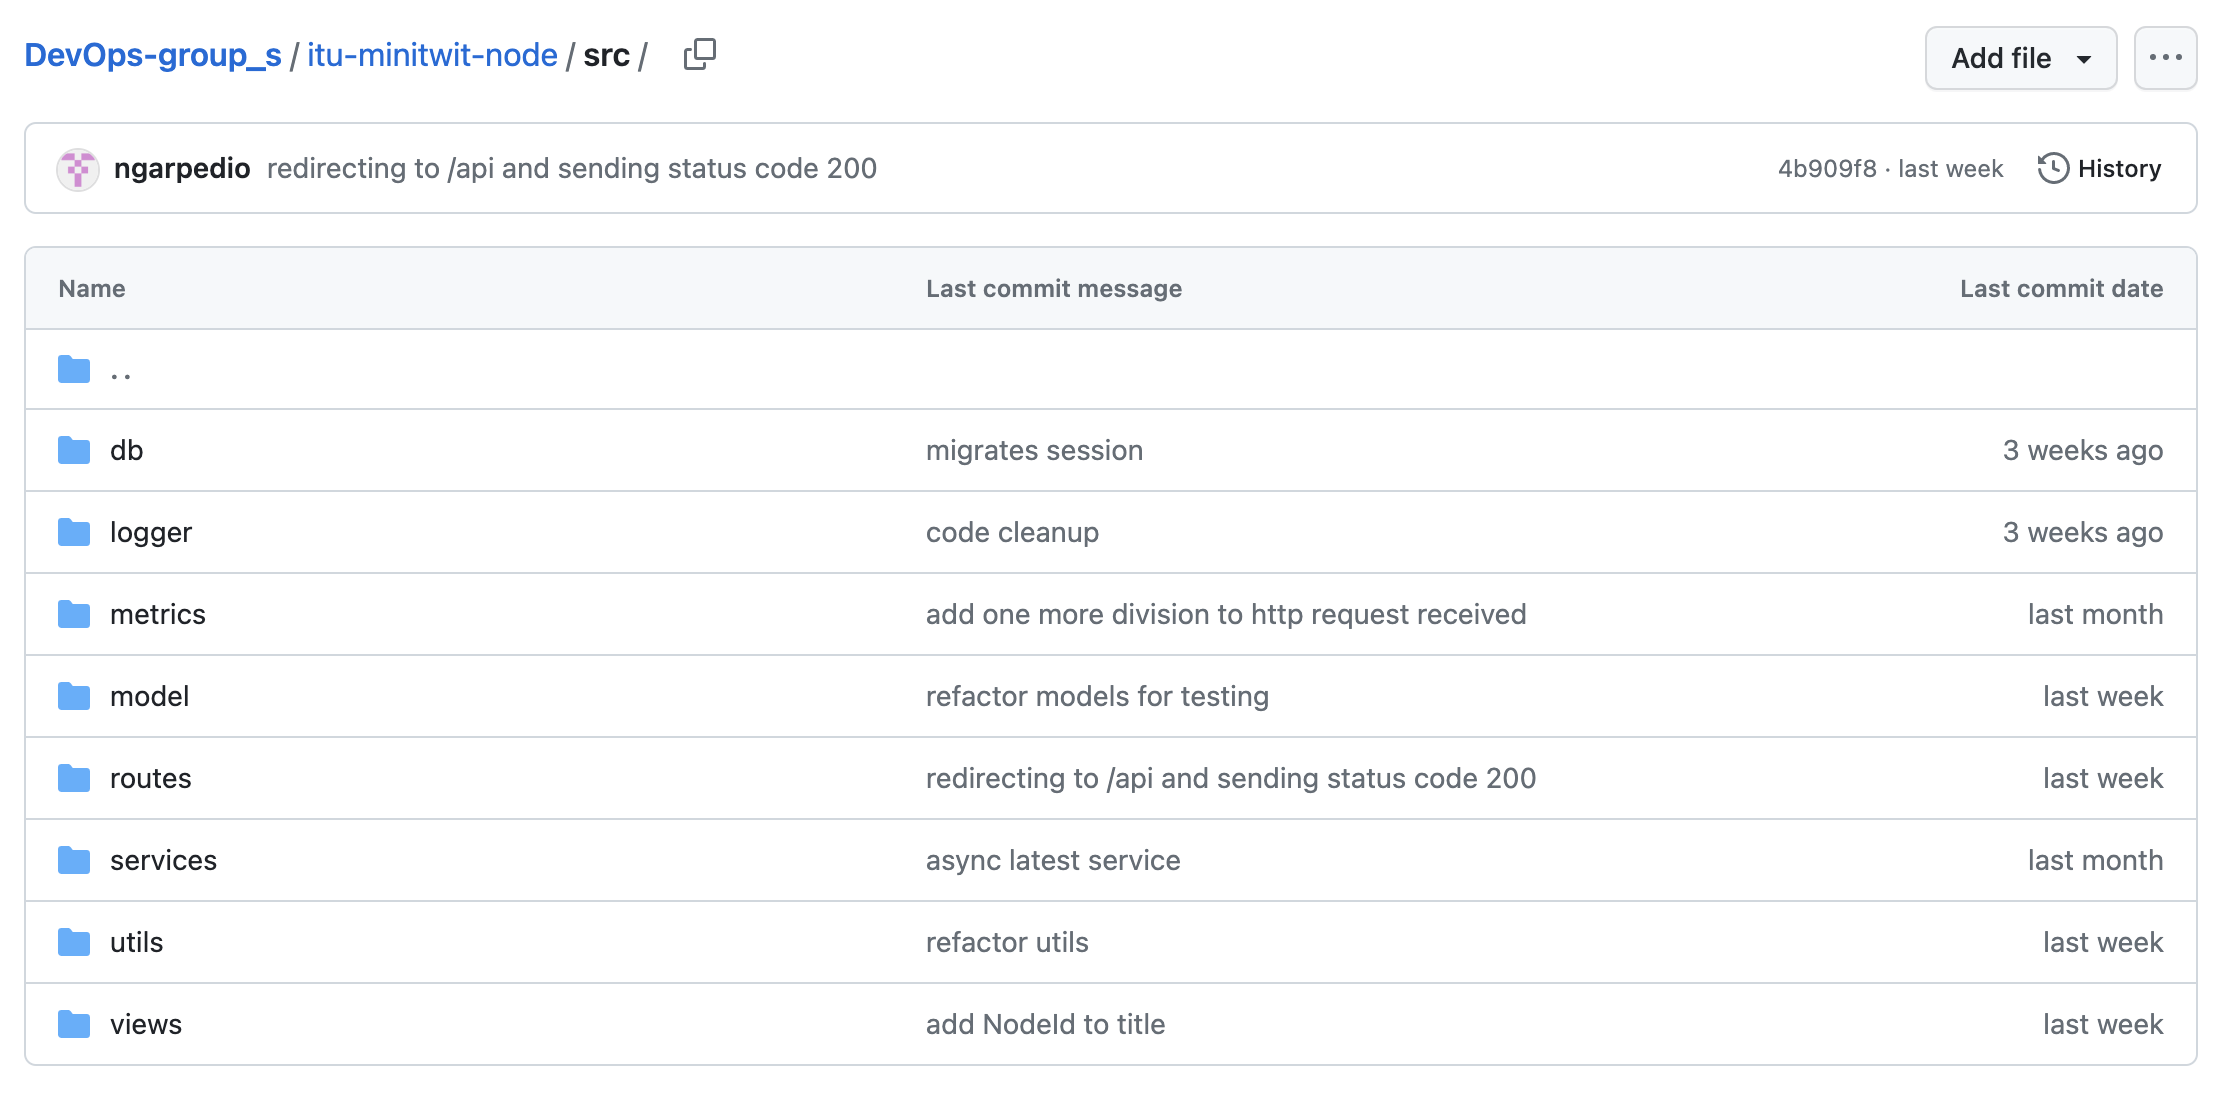
\includegraphics[width=1.15\textwidth]{images/src-folder.png} 
        \caption{\texttt{src} folder}
        \label{fig:src}
    \end{minipage}
\end{figure}

\subsection{Monitoring and logging}

\subsubsection{Monitoring}
In order to monitor our system we implemented a white box pull-based monitoring. Our implementation is rather reactive, as most of our metrics focus on the availability of our services and the infrastructure. However, we also do measure a few metrics, which give us insights into the software quality that we offer to our users. \\

In order to monitor our application and infrastructure we used Prometheus and Grafana. Prometheus is a monitoring system that scrapes our monitoring metrics every 15 seconds. The infrastructure monitoring metrics include the status of our Minitwit application and database, the uptime of the deployed containers, and memory usage. The application monitoring metrics consist of tracking the total count of HTTP errors and the error counts per individual endpoints, the number of active requests over time, and the response time of each endpoint. To collect those metrics, we instrumented our code with the \texttt{prom-client}, a Prometheus client library for Node.js applications. Grafana is a visualization web application, that was used to visualize gathered metrics in organized dashboards.

\subsubsection{Logging}
We chose to implement an EFK stack and use the Winston logging library \cite{winston} in combination with an ECSFormat module to log every HTTP request. We sort the messages based on their error level and write them into corresponding files. The log files are then continuously checked by Filebeat, which takes new entries and ships them to ElasticSearch where they are stored. Lastly, we use Kibana to query and visualize the data.\\

To test that our logging implementation works, we simulated a faulty sign-up request. We proceeded by sending a \texttt{/POST request} without providing any password value in the body. An \texttt{[ERR\_INVALID\_ARG\_TYPE]} error was logged, indicating that the implementation was working. A postmortem report of the incident has been written and added to the repository. The error can also be seen in Kibana, see Figure \ref{fig:kibana-bug}.

\begin{figure}[H]
    \centering
    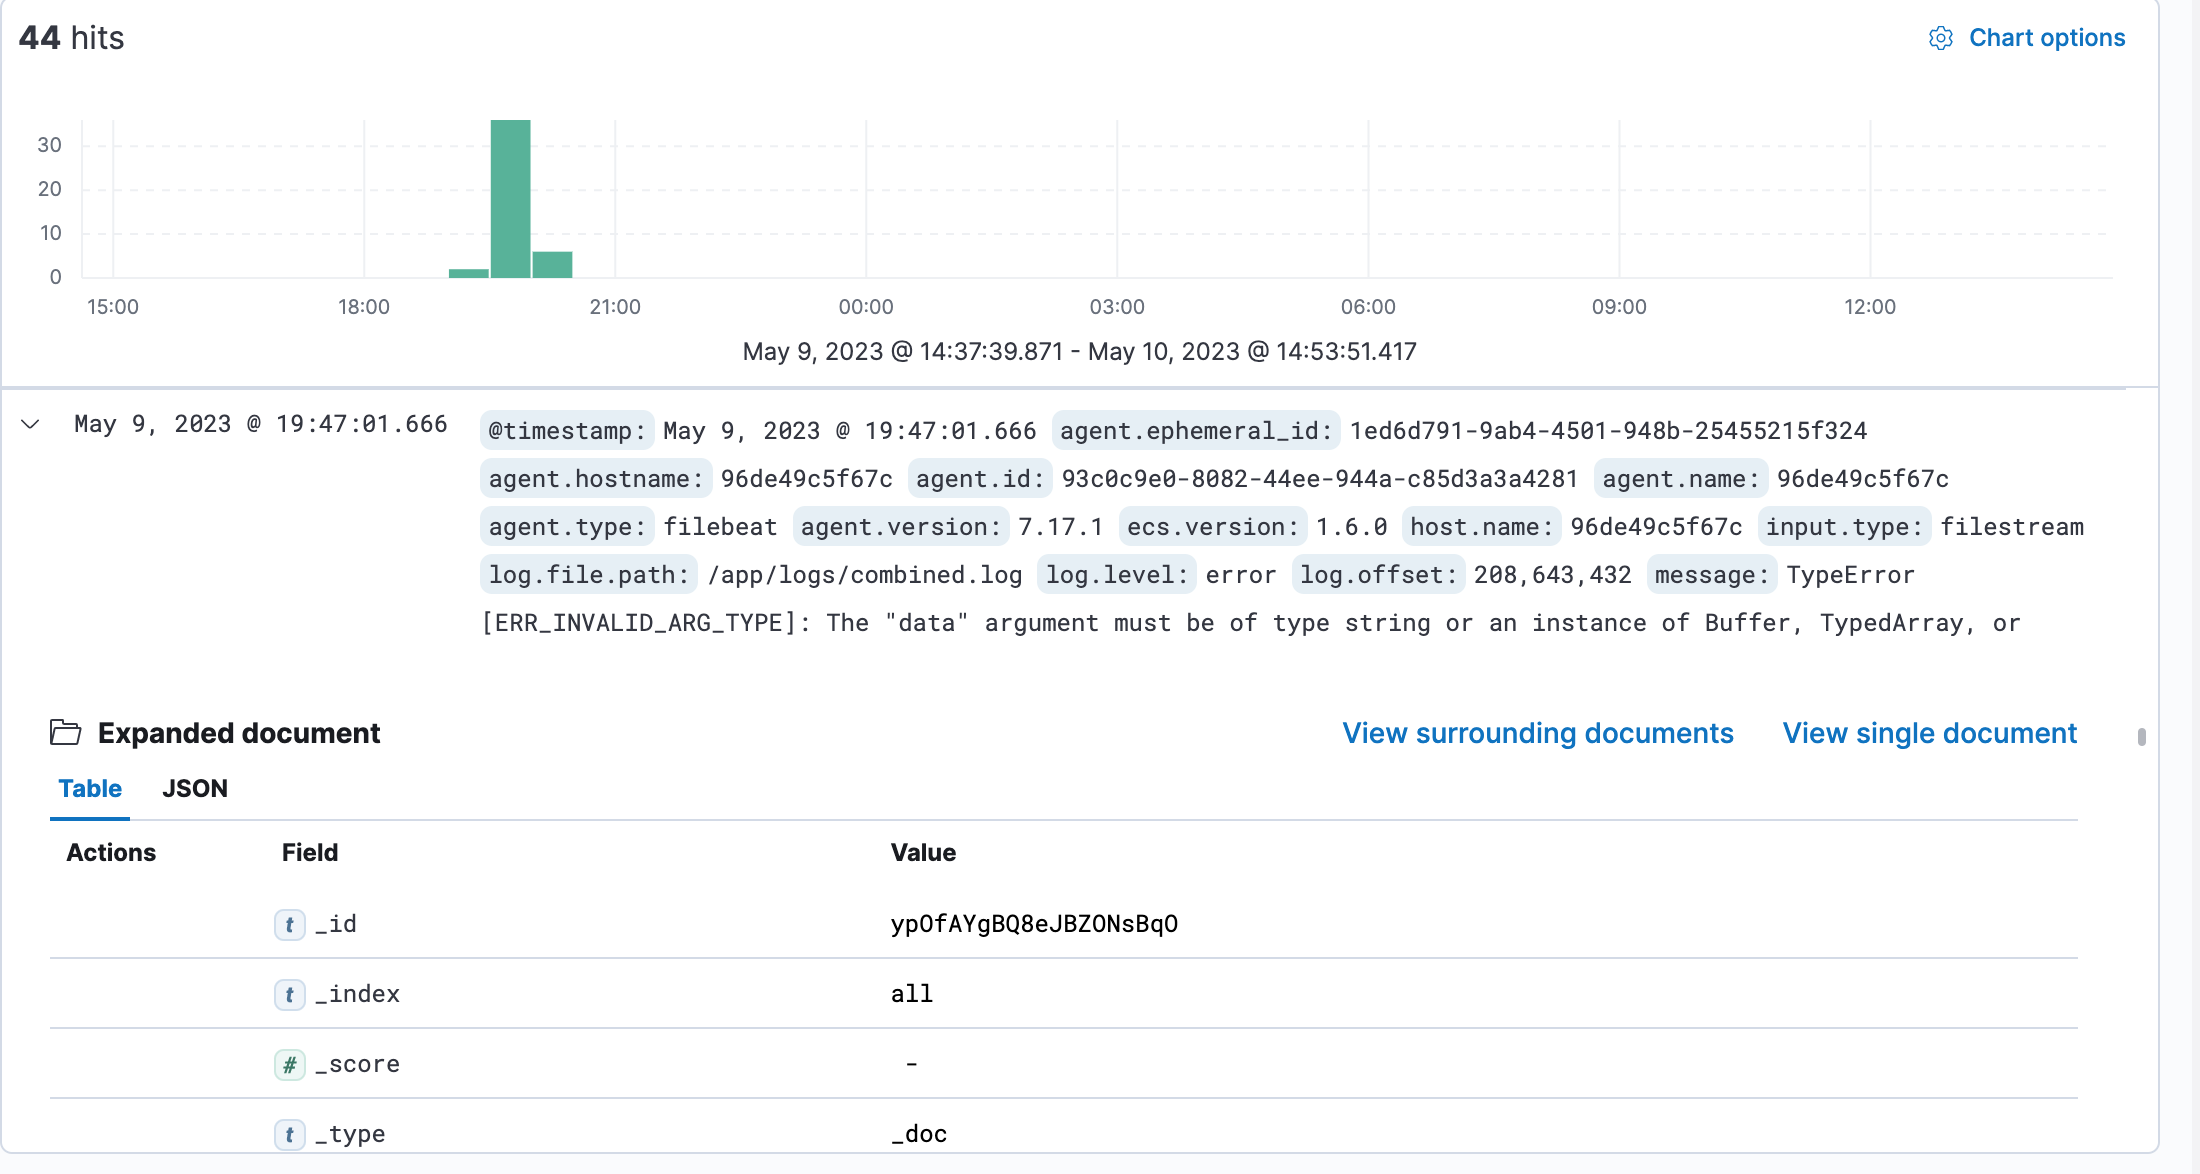
\includegraphics[width=\linewidth]{images/kibana-bug.png} 
    \caption{Error display in Kibana}
    \label{fig:kibana-bug}
\end{figure}

%Brief results of the security assessment.
\subsection{Security assessment}

\subsubsection{Risk identification}

The following assets have been identified and considered when making the security assessment:

\begin{itemize}
    \item User data: We store sensitive user information, such as emails and passwords
    \item Source code: The entire codebase of MiniTwit
    \item Production VMs: The servers utilized for running the MiniTwit application
    \item Logging data: Logs could potentially be misused to exploit the system
    \item Employees: Employee knowledge regarding the system and access credentials to various platforms
\end{itemize}

Based on the assets, we have composed seven security breach scenarios. For each scenario, the potential impact has been described and they have been categorized in terms of the three characteristics of security as defined in the CIA triad: Confidentiality, Integrity, and Availability\cite{bass2003software}. 

\begin{multicols}{2}
\begin{enumerate}

    \item \textbf{Third-party software contains malicious code or vulnerabilities}\\
    \textit{Impact:} Software vulnerabilities, data leaks \\ 
    \textit{Principle:} Integrity\\

    \item \textbf{Denial-of-service/distributed-denial-of-service attack}\\
    \textit{Impact:} Slowing down or bringing down systems \\ 
    \textit{Principle:} Availability\\

    \item \textbf{Brute-force attack}\\
    \textit{Impact:} Unauthorized access to user accounts, data leaks, manipulation of data \\
    \textit{Principle:} Confidentiality\\

    \item \textbf{SQL-injections}\\
    \textit{Impact:} Altering and/or destruction of data \\
    \textit{Principle:} Integrity

    \columnbreak
    
    \item \textbf{Man-in-the-middle attack (non-encrypted traffic)}\\
    \textit{Impact:} Data leaks \\
    \textit{Principle:} Integrity\\

    \item \textbf{Social engineering, ex. phishing e-mails}
    \textit{Impact:} Leak of company secrets, Leak of source code \\
    \textit{Principle:} Integrity\\

    \item \textbf{Attackers gain access to production VMs}\\
    \textit{Impact:} Unauthorized access, data leaks, bringing down systems \\
    \textit{Principle:} Integrity, Confidentiality,\\ Availability\\

\end{enumerate}
\end{multicols}

\subsubsection{Risk analysis and mitigation}

To determine the severity of each of the threats, we have placed them in a risk matrix to prioritize appropriate mitigation strategies. The severity categories are defined as: 
\begin{itemize}
    \item \textit{Insignificant:} Little to no impact 
    \item \textit{Marginal:} Manageable impact 
    \item \textit{Critical:} Difficult to recover
\end{itemize}

% edit figure here: https://docs.google.com/spreadsheets/d/1ZbBqvNd7IwXnbr_XMPb_ZFBBh0VcDOr2BV_DMQ8cIYg/edit?usp=sharing 
\begin{figure}[H]
    \centering
    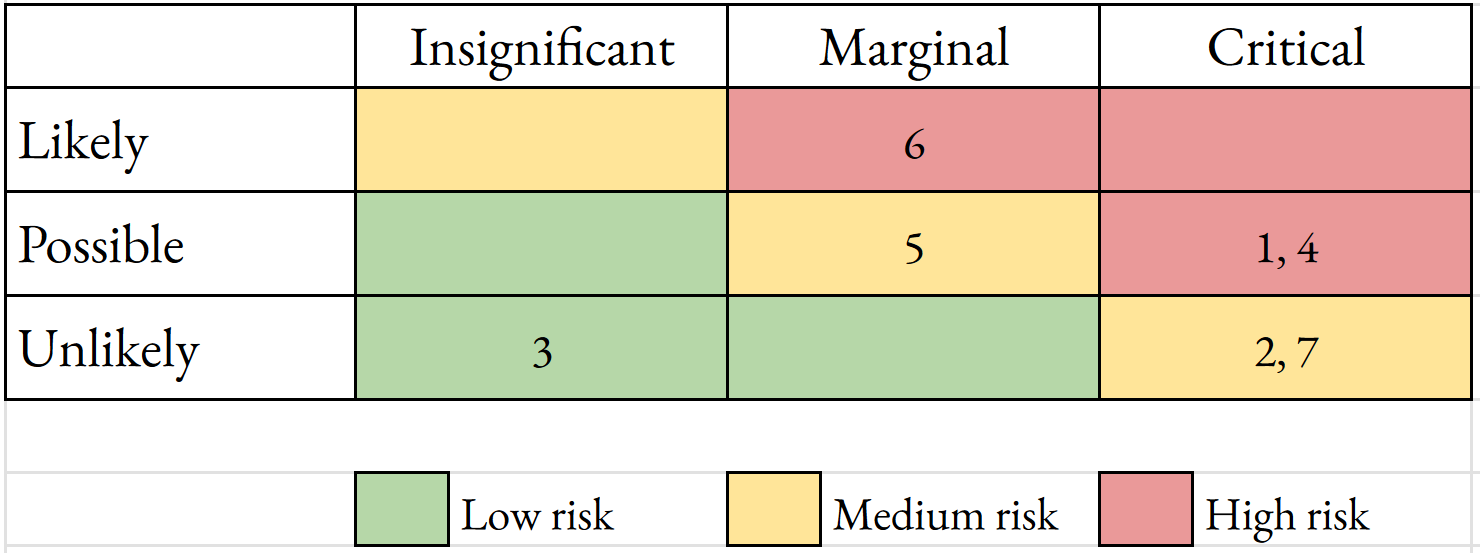
\includegraphics[width=.5\linewidth]{images/risk-matrix.png}
    \caption{Risk matrix with ids of threats.}
    \label{fig:risk}
\end{figure}


\noindent \textbf{High risk}\\
\indent \textbf{1)} The impact of a third-party vulnerability can vary broadly. Fortunately, this risk is also easy to mitigate, as static checks such as Snyk \cite{snyk} are able to identify which third-party libraries should be updated or removed.\\ 

\textbf{4)} In the worst case, SQL injections can destroy whole databases. the way we mitigated this risk was to implement an ORM framework, which abstracts away pure SQL from the source code. Further, it is possible to get automatic regular backups on your managed database in DigitalOcean.\\ 
    
\textbf{6)} This type of attack has many forms, is one of the most common, and can be almost impossible to mitigate fully. However, awareness of the potential dangers of phishing e-mails, unknown USB keys, etc. among employees is vital.\\  

\noindent \textbf{Medium risk}\\
\indent \textbf{2)} A distributed denial-of-service attack (DDoS) can bring down a system. Since it is distributed, it can be hard to detect. DigitalOcean takes some precautions in protecting against reflective DDoS attacks \cite{ddos_digitalocean}. However, we have not implemented any additional precautions.\\  
    
\textbf{5)} This risk can be mitigated through the simple use of HTTPS encryption. Due to lack of time, however, this risk has not been mitigated in Minitwit.\\ 

\textbf{7)} DigitalOcean allows firewall rules that protect access to virtual machines. However, we have not enforced any additional rules that protect our VMs.\\

\noindent \textbf{Low risk}\\ 
\indent \textbf{3)} Currently, it is possible to guess a user's password through brute force. If we were to mitigate this risk, two-factor authentication could be implemented.

\subsubsection{Automatic vulnerability test}
To test for vulnerabilities in our system, we used the tool OWASP ZAP \cite{owasp_zap}. It takes a URL as input and scans the web app for vulnerabilities. ZAP found seven vulnerabilities in our system - four marked as "medium" risk, and three marked as "low" risk. The alerts can be seen in Figure \ref{fig:zap-alerts}.

\begin{figure}[H]
    \centering
    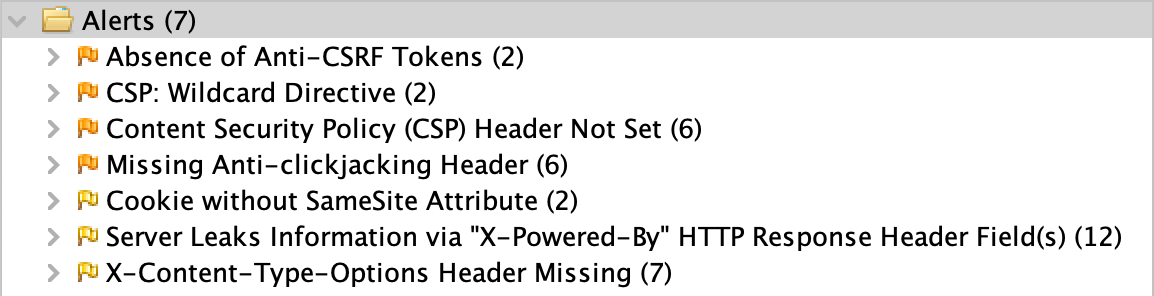
\includegraphics[width=.6\linewidth]{images/zap-alerts.png}
    \caption{The security alerts identified by OWASP ZAP.}
    \label{fig:zap-alerts}
\end{figure}

We decided to focus on the alert \textit{"Server Leaks Information via 'X-Powered-By' [...]"}. Here, ZAP tells us that frameworks used by our application will be visible in HTTP response headers. It means that attackers could potentially check for vulnerabilities in these frameworks and use them to their advantage. The 'X-Powered-By' field can easily be omitted by including the line "\texttt{app.disable('x-powered-by');}" in our \texttt{app.js} file. However, we decided to include the Helmet dependency \cite{helmet} instead, as it includes an array of response header protection, not just on the 'X-powered-by' field. We were able to see traces of the ZAP scan in our EFK stack, seen in Figure \ref{fig:kibana-logs-zap}, which shows a spike in activity for a few seconds (the scan was done after the simulator was shut down).

\begin{figure}[H]
    \centering
    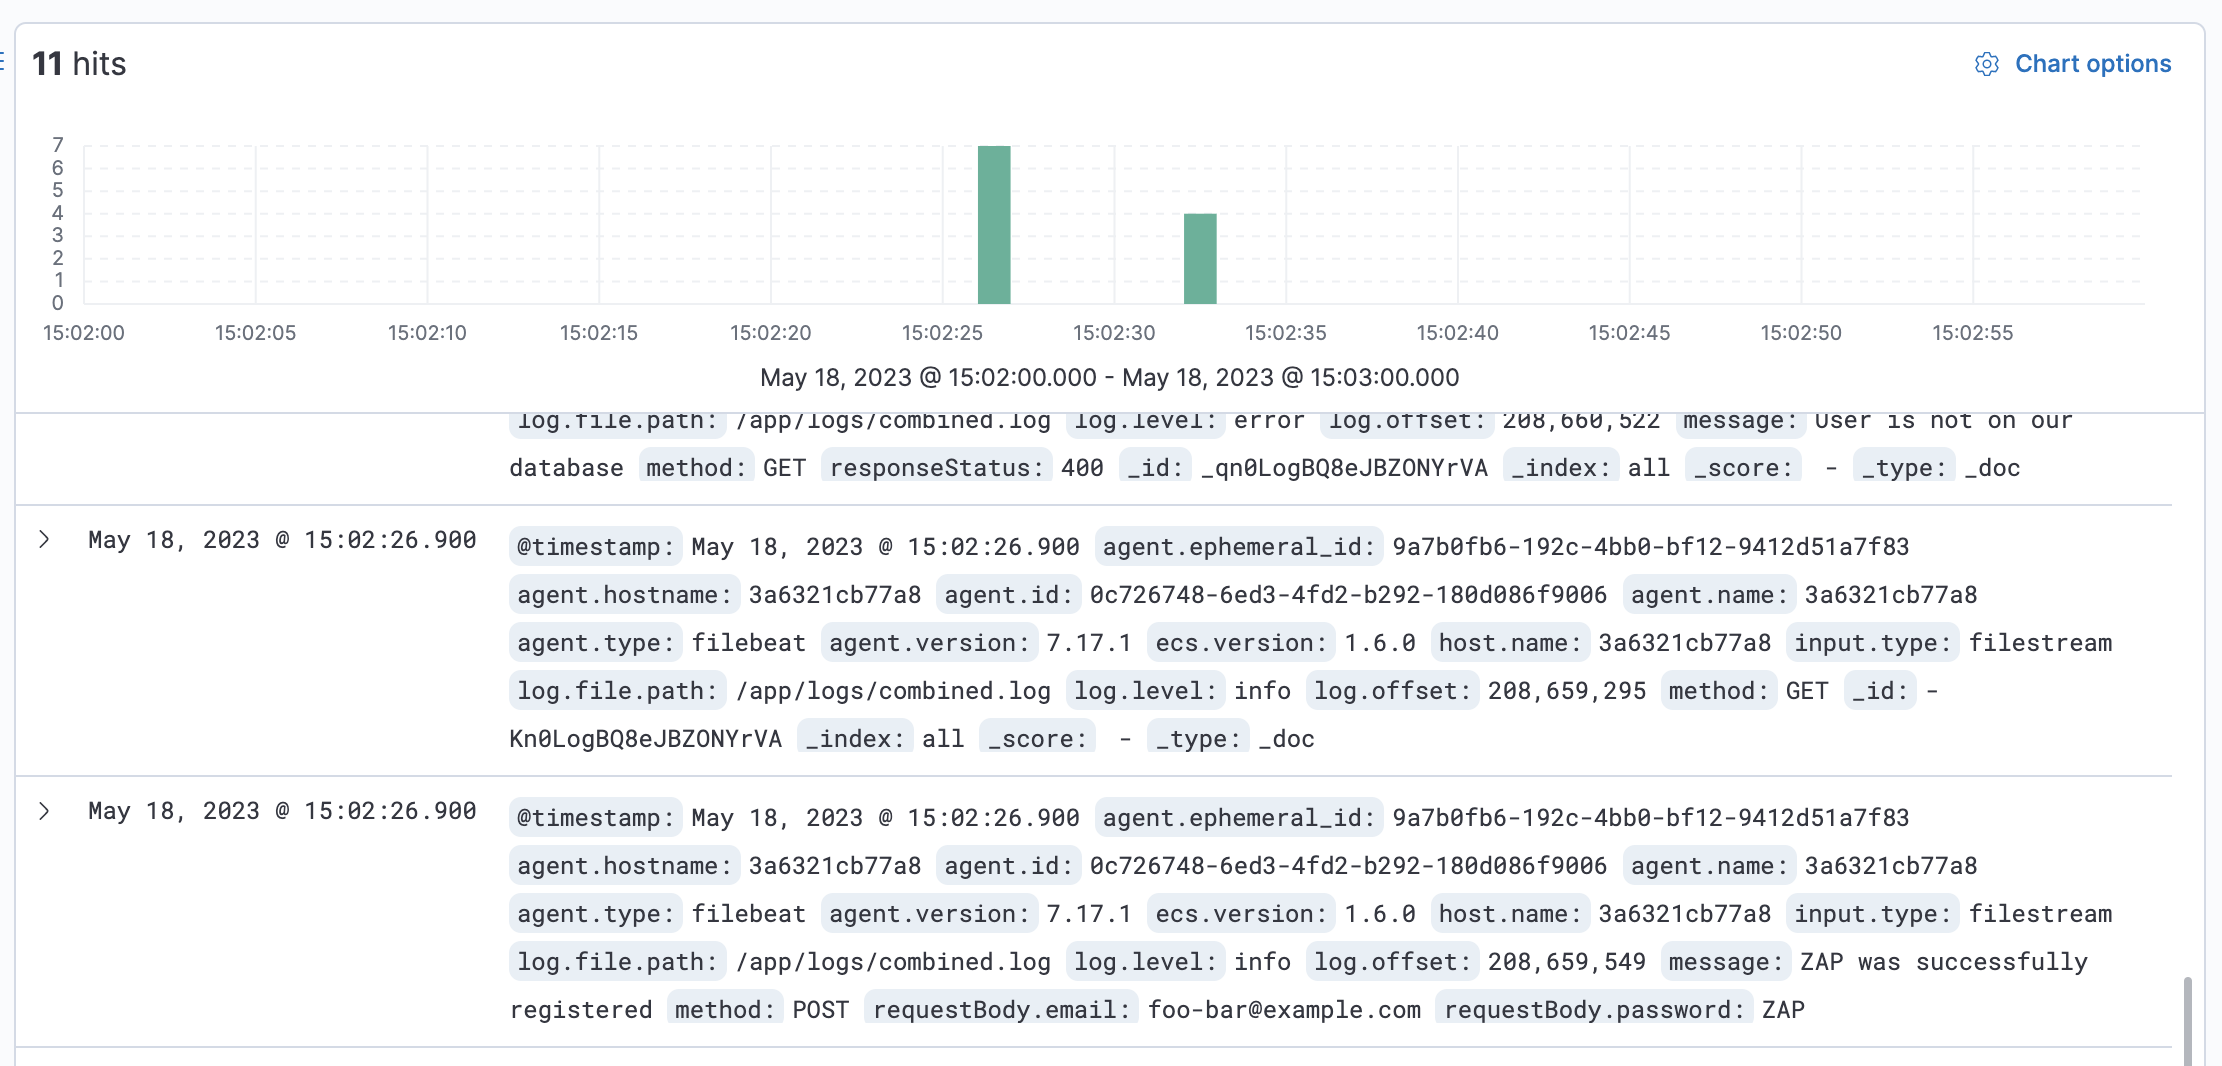
\includegraphics[width=\linewidth]{images/kibana-zap-logs.png}
    \caption{Activity in the logs after running a security scan with OWASP ZAP.}
    \label{fig:kibana-logs-zap}
\end{figure}

% What does the Zap test look like now?

We would have liked to run the OWASP ZAP check once again after including the Helmet dependency. However, we had to shut down the app before running ZAP again to avoid receiving a large bill from DigitalOcean. 


\subsection{Scaling and load balancing strategy}
%Applied strategy for scaling and load balancing.
\subsubsection{Scaling and Docker Swarm}
Although DigitalOcean makes it easy to scale applications vertically by increasing droplet size, we decided to scale our system horizontally using Docker Swarm \cite{docker_swarm}. We decided on Docker Swarm mode as it allows for container orchestration, which is something we wanted to get experience with. In addition, Docker Swarm includes capabilities like self-healing (restarting services when they are down) and built-in load balancing. The cluster is built in code using Terraform\cite{terraform}. The \texttt{main.tf} file sets up one leader (manager) droplet, one manager droplet, and two worker droplets in DigitalOcean. The \texttt{minitwit\_stack.yml} file sets up services for the cluster. All services are in replicated mode, with three replicas of \texttt{minitwit}, two replicas of \texttt{filebeat}, and a single \texttt{flagtool}. Here, we also add additional services: a Docker Swarm Visualizer and an NGINX load balancer. If we need to scale up the capacity of our application in the future, we can simply rewrite the Terraform file and redeploy it.

\subsubsection{Load balancing}
Adding an NGINX load balancer in our stack file means that we not only have load balancing between nodes but also "in front of" the whole cluster. While the NGINX load balancer distributes task load to an appropriate node, the ingress load balancer in each node makes sure that a request to a specific service will be rerouted to the node running that service. The current system does not use HTTPS for secure client-server communication. However, if we were to implement that in the future, an added bonus of having an extra load balancer is that only traffic to and from that load balancer would need to be secure, as all other communication would run within a closed system. 

\subsection{Use of AI-assistants}
We used two different AI assistants during the project: GitHub Copilot and ChatGPT. A few of the team members used GitHub Copilot as a code assistant. This speeds up the coding process, particularly during the initial phase of rewriting the application from Flask to Express.js. ChatGPT was used by all team members and used more as an occasional helper when stuck with a code or a configuration problem. Its effectiveness varied, occasionally leading to confusion. We observed that ChatGPT is more adept at providing general code structures rather than specific configurations. If ChatGPT was used for any sections of the report, we have mentioned it in the relevant section. 

%In case you have used AI assistants for writing code during your project or to write the report:
%Explain which system(s) you used during the project.
%Reflect on how it supported/hindered your process.
%In essence it has to be clear how code or other artifacts come from idea into the running system and everything that happens on the way.

\section{Lessons Learned Perspective}
%Describe the biggest issues, how you solved them, and which are major lessons learned with regards to: evolution and refactoring, operation, and maintenance
%Also reflect and describe what was the "DevOps" style of your work. For example, what did you do differently in previous development projects and how did it work?

% ~~~ STRUCTURE ~~~~ 
% Heading: A short key phrase capturing the topic. This is a title, not a sentence. Try to make it concise and relevant.

%Brief statement on the learning: What is the learning? 

%Recollection of the event(s): What triggered the learning? 

%Impact and implications of the observed event(s): This part could be a reflection or an analysis of the situation. It is not uncommon to have this part mixed with the previous point. It is better if you can separate it.

%How will this learning influence future participation in the project: This part is optional and is usually present in outstanding diaries.

\subsection{Lack of holistic view of the system}
Only very late in the project did we learn the advantage of the first way of DevOps: flow \cite{kim2021devops}. When the simulator was started, our system was lacking behind in various ways. However, instead of doing little by little and bettering the system as a whole, we did everything we could to adhere to the simulator's API. As a result, we ended up migrating the database and implementing the ORM framework a lot later in the project than intended. Had we simply accepted that the simulator endpoints would not be perfect from the start, the system could have gradually gotten better.

\subsection{Better refinement of tasks}
We maintained an updated Kanban board by transferring tasks from the weekly project work assignments. However, we frequently encountered situations where seemingly straightforward tasks ended up taking more time than anticipated. We believe that this could have been alleviated by collaboratively refining the tasks. By utilizing the collective knowledge of the team, we could have cooperatively written solution keywords that potentially could have optimized our work. Additionally, this approach would have facilitated continuous learning, which is the third way of DevOps\cite{kim2021devops}, as everyone would have gained a better overview and a basic understanding of all tasks, rather than just the ones they were individually responsible for. 

\subsection{Earlier implementation of proper CI/CD pipelines}
We have learned how properly implemented CI/CD pipelines significantly improve the flow of development in projects. As mentioned, 
we did not manage to integrate tests and separate our pipelines until late in the project. This resulted in multiple incidents of pushing faulty code to our \texttt{main} branch and it made it difficult to test additions to the pipelines since it would not be triggered until pushing to \texttt{main}. Since succeeding in separate pipelines, we have experienced the value of increased branch protection and a shorter feedback loop.  

\subsection{Single owner of our GitHub repository}
During the course of the project, our repository was set up with a single owner, which means only a single team member could change code secrets, repository settings, and permissions. Not only did this lead to bottlenecks a few times in the project, but it also made the project feel slightly less agile. Alternatively, we could have created a company GitHub repository with equal permissions between members. 

\subsection{Good practices even with tight deadlines}
Towards the end of the project, we ended up slacking on a few of the practices we had originally committed to, for example, our pull request practice. At certain points when we needed to do a lot of changes in a short amount of time, we ended up committing small fixes directly to \texttt{main} instead of going through a pull request of a feature branch. Although it did not end up breaking anything, it is bad practice and something we brought back into internal feedback, following the second way of DevOps \cite{kim2021devops}. Here at the end, we are back to our original branching strategy and pull request practices. 

\subsection{Individual learning on DevOps in general}
Evaluating the lessons learned from a higher perspective than simply the project, the DevOps course positively affected our individual learning of what DevOps means to a project or an organization. Working with both theory and practice on IT infrastructure and development has challenged all of us. It truly led to new perspectives and enhanced our problem-solving abilities. Most importantly, it truly helped us “bridge the gap between Development and Operations, emphasizing communication and collaboration" \cite{jabbari2016devops}. 


%\subsection{Conclusion on learning}
%Evaluating the lesson learned from a higher perspective than this project, the DevOps course positively affected our learning behavior. Especially in relation to IT infrastructures and development, each one of us was challenged with new learnings. Each of these learnings contributed to enhancing our problem-solving ability, and most importantly  “to bridge the gap between Development and Operations, emphasizing communication and collaboration.." \cite{jabbari2016devops}. 


%We consider the Three ways of DevOps, explained in the "The DevOps Handbook" \cite{kim2021devops}. The three ways can be summarised by 1) optimizing the value stream by understanding the whole system, 2) learning from failures and having feedback loops to fix issues quickly, and 3) continuous experimentation and learning, empowering the team’s individuals. 

%We decided to evaluate our efforts based on the different sets of operations in the project: evolution, refactoring, and maintenance, and apply them to two macro areas. The first area of reflection tackles the unbalanced way of focusing on the tasks which affected the quality of our product. The second area considers the excess of confidence when confronting ourselves with new learnings, resulting in “almost” catastrophic slowdowns.\\

%\subsection{Overfocus on one part of our project}
%One of the main lessons that we learned was to always focus on the whole system. As we put too much focus on the simulator, at the beginning, which led to a few undesirable situations. One example was our approach to query optimization. We were so concerned about having the simulator running seamlessly, that we optimized our database and queries to only the simulator’s purposes. We completely neglected the UI part of our system, reaching a point, where displaying “my timeline” would take a minute. By this, we were not adhering to the first way of DevOps, which says that it is crucial to ensure a smooth and efficient transition of code and changes from development to operations. This includes optimizing all aspects of the system. This aspect was something, that we learned only in the later stages of the development process. Neglecting other parts was reflected also in our initial CI/CD implementation, as we included tests, whose main focus was on testing the simulator endpoint logic and operations. This resulted in a few situations when we pushed a code, that introduced bugs into our production code. This was breaking the second way of DevOps, as we did not have comprehensive feedback loops allowing us to fix all issues quickly. All these problems led to a realization, that we need to shift focus to the whole system again because neglecting other parts of the system was hindering the overall flow and performance. By overlooking other parts, we may inadvertently impede the speed and effectiveness of the development-to-operations pipeline. Most importantly, we used these problems as a learning experience to improve, which adheres to the third way of DevOps.\\

%\subsection{Wrong time estimation and confidence}
%Fostering a culture of continuous experimentation and enabling each one of us to take risks and embrace failure is what the third way of DevOps expresses \cite{kim2021devops}. When trying to implement the CI/CD chain through GitHub Actions, one of our biggest issues was an overconfident approach. The time spent completing the task resulted to be much longer than what was initially assessed. The CI/CD example was not the only one where we experienced such “slowdowns”. Other examples are also database migration and the implementation of the swarm. As no one in the group was an expert in the tools and processes used in the project, we took the experience as valuable learning. Through these endeavors, our ways of working are linked with Devops’ second way, where feedback helps to understand the root causes of the issues, learn from incidents, and solve problems preventing the successful delivery of our product. Contrary to the first Way of DevOps, which consists of including a flow that quickly connects developments to operations in order to optimize value, the CI/CD implementation was treated as a standalone task that could have been cut into smaller components and tackled individually.\\

%\subsection{Conclusion on learning}
%Evaluating the lesson learned from a higher perspective than this project, the DevOps course positively affected our learning behavior. Especially in relation to IT infrastructures and development, each one of us was challenged with new learnings. Each of these learnings contributed to enhancing our problem-solving ability, and most importantly  “to bridge the gap between Development and Operations, emphasizing communication and collaboration.." \cite{jabbari2016devops}. 

\newpage

\setcitestyle{square} % change citations to appear in [] instead of ()
\bibliographystyle{plain}
\bibliography{references}

\newpage
\section{Appendix}

%All dependencies of your ITU-MiniTwit systems on all levels of abstraction and development stages. That is list and briefly describe all technologies and tools you applied and depend on.

\subsection{List of dependencies}
\label{app:dependencies}

\noindent The descriptions of the list of dependencies have been partly written by ChatGPT.\\ 

\textbf{Frontend}
\begin{itemize}
    \item \texttt{jade 1.11.0}: (now known as Pug) template engine for NodeJS\\
\end{itemize}

\textbf{Backend}
\begin{itemize}
    \item \texttt{cookie-parser 1.4.4}: a middleware for Express that parses HTTP request cookies and makes them available in your application's request object
    \item \texttt{crypto 1.0.1}: a Node.js module that provides cryptographic functionality - used with gravatar
    \item \texttt{dotenv 16.0.3}: a zero-dependency module that allows you to store configuration variables in a file and easily access them in your application
    \item \texttt{express 4.16.1}: web application framework for Node.js that provides a set of features and middleware to build web servers and APIs
    \begin{itemize}
        \item \texttt{express-mysql-session 3.0.0}: a session store for Express applications that uses MySQL to store session data
        \item \texttt{express-session 1.17.3}: a middleware for session management in Express applications that provides session handling capabilities
    \end{itemize}
    \item \texttt{helmet 7.0.0}: a middleware for securing Express applications by setting various HTTP headers to prevent common security vulnerabilities
    \item \texttt{mysql2 3.3.0}: a MySQL client for Node.js
    \item \texttt{Node.js 18.14.0}: an open-source, server-side runtime environment that allows you to execute JavaScript code outside of a web browser
    \item \texttt{nodemon 2.0.20}: a utility that monitors changes in your Node.js application's files and automatically restarts the application when changes occur
    \item \texttt{os 0.1.2}: a Node.js module that provides operating system-related functionality 
    \item \texttt{path 0.12.7}: a Node.js module that provides utilities for working with file paths
    \item \texttt{url 0.11.0}: a Node.js module that provides utilities for URL handling and manipulation
    \item \texttt{winston 3.8.2}: a versatile logging library for Node.js.
    \item \texttt{sequelize 6.31.1}: a JavaScript ORM framework\\
    
\end{itemize}

\textbf{Testing}
\begin{itemize}
    \item \texttt{chai 4.3.7}: assertion library for JavaScript testing
    \item \texttt{cypress 12.10.0}: JavaScript testing framework for E2E and UI testing
    \item \texttt{debug 2.6.9}: debugging utility for Node.js applications
    \item \texttt{mocha 10.2.0}: a JavaScript testing framework for Node.js applications
    \item \texttt{sinon 15.0.4}: a JavaScript testing library that provides test spies, stubs, and mocks
    \item \texttt{supertest 6.3.3}: library for HTTP request testing\\
\end{itemize}

\textbf{Other development and collaboration technologies}
\begin{itemize}
    \item \texttt{@elastic/ecs-winston-format 1.3.1}: library that provides a log formatter that logs entries according to the Elastic Common Schema (ECS) format
    \item \texttt{npm 9.4.2}: a Node.js package manager
    \item \texttt{prom-client 14.2.0}: a Prometheus client library for Node.js. It provides an API to instrument your applications and expose metrics that can be scraped by Prometheus for monitoring and alerting
    \item \texttt{docker}: A platform for containerization that allows developers to package and distribute applications with their dependencies.
    \item \texttt{docker-compose}: A tool for defining and running multi-container Docker applications, simplifying the management of complex, interconnected services.
    \item \texttt{git 2.40.1}: A distributed version control system that enables developers to track and manage changes to source code efficiently. 
    \item \texttt{grafana 8.1.5}: A data visualization and monitoring tool that helps users analyze and display metrics from various data sources.
    \item \texttt{kibana}: A web interface that allows users to explore, visualize, and analyze data stored in Elasticsearch using charts, graphs, and dashboards.
    \item \texttt{filebeat 7.17.1}: A lightweight log shipper that forwards log files from various sources to Logstash or Elasticsearch for centralized log management.
    \item \texttt{terraform}: An infrastructure-as-code tool that enables users to define and provision infrastructure resources across various cloud providers and services.
    \item \texttt{snyk}: A security tool that identifies vulnerabilities and provides remediation guidance for open-source libraries and container images.
    \item \texttt{sonarcloud}: A cloud-based code quality and security platform that analyzes source code for bugs, vulnerabilities, and code smells.
    \item \texttt{owasp-zap 2.12.0}: An open-source web application security scanner that helps identify security vulnerabilities during the development and testing phases.
\end{itemize}

\end{document}
